\documentclass[12pt,a4paper]{report}

% ------------------------------------------------------------------
%  Root document — assembles the thesis from its parts:
%    preamble.tex (packages, page geometry, heading styles, etc.)
%    metadata.tex (thesis-specific data: title, author, abstracts)
%    front-matter.tex (cover-page / abstract-page templates)
%    chapters/ (one file per chapter)
%    appendix/ (appendix content)
% ------------------------------------------------------------------
% ============================================================
%  PREAMBLE
%  All package loading and document-wide formatting lives here.
%  Thesis content (title, author, abstracts) is in metadata.tex.
%  Cover-page / abstract-page layouts are in front-matter.tex.
% ============================================================

% --- Encoding & language ---
\usepackage[romanian]{babel}
\renewcommand\familydefault{\sfdefault} % sans-serif as the body font
\addto\captionsromanian{
    \renewcommand{\appendixname}{Anexa}
    \renewcommand{\chaptername}{Capitolul}
    \renewcommand{\contentsname}{Cuprins}
    \renewcommand{\figurename}{Figura}
    \renewcommand{\tablename}{Tabelul}
}

% --- Page geometry ---
\usepackage[margin=2.54cm]{geometry}

% --- Graphics ---
\usepackage{graphicx}

% --- Chapter / section heading style ---
\usepackage{titlesec}
\titleformat{\chapter}{\large\bfseries\MakeUppercase}{\thechapter}{2ex}{}
\titlespacing*{\chapter}{0pt}{0pt}{1ex}
\titleformat*{\section}{\large\bfseries}
\titleformat*{\subsection}{\large\bfseries}
\titleformat*{\subsubsection}{\large\bfseries}

% --- Appendix support ---
\usepackage[titletoc,title]{appendix}

% --- Continuous numbering of figures/tables/equations across chapters ---
\counterwithout{figure}{chapter}
\counterwithout{table}{chapter}
\counterwithout{equation}{chapter}

% --- Tables, arrays, lists ---
\usepackage{booktabs}
\usepackage{array}
\usepackage[inline]{enumitem}
\setlist{noitemsep}

% --- Code listings ---
\usepackage{listings}

% --- Misc text utilities ---
\usepackage{verbatim} % comment environment for blocking out source

% --- Headers & footers ---
\usepackage{fancyhdr}
\pagestyle{empty} % front matter: no header/footer decoration
\renewcommand{\headrulewidth}{0pt}
\renewcommand{\footrulewidth}{0pt}
\fancyhf{} % clear all six header/footer fields
\cfoot{\thepage}

% --- Hyperlinks & cross-references ---
% Load order is strict: cite → hyperref → xurl → microtype → subcaption → cleveref
\usepackage{cite}
\usepackage[hidelinks]{hyperref}
\usepackage{xurl}
\usepackage{subcaption}
\usepackage[nameinlink]{cleveref}

\crefname{equation}{ecuația}{ecuațiile}
\Crefname{equation}{Ecuația}{Ecuațiile}
\crefname{figure}{figura}{figurile}
\Crefname{figure}{Figura}{Figurile}
\crefname{section}{secțiunea}{secțiunile}
\Crefname{section}{Secțiunea}{Secțiunile}
\crefname{table}{tabelul}{tabelurile}
\Crefname{table}{Tabelul}{Tabelurile}

\newcommand{\crefpairconjunction}{ și }
\newcommand{\crefmiddleconjunction}{, }
\newcommand{\creflastconjunction}{ și }
\newcommand{\crefrangeconjunction}{--}

% --- Global spacing ---
\linespread{1.15}
\setlength{\parindent}{0pt}
\setlength{\parskip}{.28cm}

% ============================================================
%  THESIS METADATA
%  Edit the values in this file for your thesis. Everything
%  else (preamble.tex, titlepages.tex) is reusable template
%  code and should not normally need to change.
% ============================================================

% --- People ---
\newcommand{\Name}{Andrei-Silviu Voicu}
\newcommand{\Advisor}{Conf. dr. ing. Cornel Popescu}

% --- Title (Romanian / English) ---
\newcommand{\ProjectTitleRO}{Platformă educațională pentru învățarea limbii engleze}
\newcommand{\ProjectTitleEN}{Educational platform for learning English}

% --- Date shown on the cover pages ---
\newcommand{\MonthRO}{IULIE}
\newcommand{\MonthEN}{JULY}
\newcommand{\Year}{2026}

% --- Abstracts ---
% Max. ~200 words each; together both versions should fit on one page.
\newcommand{\AbstractRO}{Lucrarea prezintă o platformă web pentru studiul limbii engleze. Ideea de la care s-a plecat este că majoritatea platformelor existente acoperă fie conținutul didactic, fie sesiunile live cu profesori, rareori pe ambele, ceea ce îl obligă pe utilizator să combine mai multe servicii ca să își acopere nevoile de bază. Platforma include cursuri pe trei niveluri de dificultate, exerciții și teste cronometrate, iar utilizatorii pot rezerva sesiuni cu profesori verificați pe platformă, fie individual, fie în grup, accesul la sesiuni funcționând pe baza unui sistem de credite. Profesorii nu pot preda imediat după înregistrare, ci trec printr-un proces de aprobare, iar cursurile create de aceștia sunt revizuite înainte de a apărea în catalog. Progresul fiecărui student este urmărit atât la nivel de lecție, cât și la nivel de quiz, rezultatul final fiind o aplicație care acoperă ciclul întreg de învățare, de la înregistrarea contului până la susținerea sesiunilor video.}

\newcommand{\AbstractEN}{This paper presents a web platform for learning English. The starting point was a fairly common problem: most existing platforms cover either study materials or live sessions with instructors, rarely both, which forces users to combine multiple services just to cover their basic needs. The platform includes courses across three difficulty levels, interactive exercises and timed quizzes, and users can book sessions with verified instructors, either one-on-one or in a group, with access working through a credit system tied to a subscription. Instructors cannot start teaching right after signing up, they go through an approval process, and any courses they create are reviewed before appearing in the catalog. Student progress is tracked at both the lesson and quiz level, with the end result being a functional application that covers the full learning cycle, from account registration to completing video sessions with an instructor.}

% ============================================================
%  FRONT MATTER TEMPLATE
%  Institutional boilerplate and the macros that lay out the
%  Romanian/English cover pages and the abstract page.
%
%  Nothing in this file should normally need to change between
%  theses — student-specific values (name, title, advisor,
%  abstracts) live in metadata.tex and are referenced below.
% ============================================================

\newcommand{\HeaderLineSpace}{1ex}

% --- Institution header block (Romanian / English) ---
\newcommand{\UniTextRO}{%
    UNIVERSITATEA NAȚIONALĂ DE ȘTIINȚĂ ȘI TEHNOLOGIE POLITEHNICA DIN BUCUREȘTI \\[\HeaderLineSpace]
    FACULTATEA DE AUTOMATICĂ ȘI CALCULATOARE \\[\HeaderLineSpace]
    DEPARTAMENTUL DE CALCULATOARE \\}

\newcommand{\UniTextEN}{%
    NATIONAL UNIVERSITY OF SCIENCE AND TECHNOLOGY POLITEHNICA OF BUCHAREST \\[\HeaderLineSpace]
    FACULTY OF AUTOMATIC CONTROL AND COMPUTERS \\[\HeaderLineSpace]
    COMPUTER SCIENCE AND ENGINEERING DEPARTMENT \\}

% --- Fixed labels (Romanian / English) ---
\newcommand{\DiplomaRO}{PROIECT DE DIPLOMĂ}
\newcommand{\DiplomaEN}{DIPLOMA PROJECT}

\newcommand{\AdvisorRO}{Coordonator științific:}
\newcommand{\AdvisorEN}{Thesis advisor:}

\newcommand{\BucRO}{BUCUREȘTI}
\newcommand{\BucEN}{BUCHAREST}

% --- Generic cover page ---
% \frontPage{header}{diploma label}{title}{advisor label}{city}{month}
%   #1  institution, faculty, and department block (\UniTextRO or \UniTextEN)
%   #2  diploma label (\DiplomaRO or \DiplomaEN)
%   #3  project title (\ProjectTitleRO or \ProjectTitleEN)
%   #4  advisor field label (\AdvisorRO or \AdvisorEN)
%   #5  city (\BucRO or \BucEN)
%   #6  month, printed before \Year (\MonthRO or \MonthEN)
% Student name (\Name), advisor name (\Advisor) and \Year are read directly
% from metadata.tex and are shared by both language variants.
\newcommand{\frontPage}[6]{%
    \begin{titlepage}
        \begin{center}
            {\Large #1}
            \vspace{40pt}
            
            \begin{tabular}[c]{c@{\hspace{4cm}}c}
                
\includegraphics[scale=0.015]{pics/logos/unstpb-logo.png} &
                
\includegraphics[scale=0.15]{pics/logos/cs-logo.jpg}
            \end{tabular}
            
            \vspace{105pt}
            {\Huge #2}\\
            \vspace{20pt}
            {\Large #3}\\ 
            \vspace{50pt}
            {\LARGE \Name}\\
        \end{center}
        
        \vfill
        \begin{tabular*}{\textwidth}{@{\extracolsep{\fill}}p{6cm}r}
            & {\large\textbf{#4}}\\[10pt]
            & {\large \Advisor}
        \end{tabular*}
        
        \vspace{20pt}
        \begin{center}
            {\large\textbf{#5}}\\
            {\normalsize #6 \Year}
        \end{center}
    \end{titlepage}%
}

\newcommand{\frontPageRO}{%
    \frontPage{\UniTextRO}{\DiplomaRO}{\ProjectTitleRO}{\AdvisorRO}{\BucRO}{\MonthRO}}

\newcommand{\frontPageEN}{%
    \frontPage{\UniTextEN}{\DiplomaEN}{\ProjectTitleEN}{\AdvisorEN}{\BucEN}{\MonthEN}}

% --- Abstract page (Romanian "SINOPSIS" + English "ABSTRACT") ---
\newcommand{\AbstractPage}{%
    \begin{titlepage}
        \textbf{\large SINOPSIS}\par
        \AbstractRO\par\vfill
        \textbf{\large ABSTRACT}\par
        \AbstractEN\vfill
    \end{titlepage}%
}


% While working on a single chapter, uncomment the next line to only
% typeset that chapter (others are pulled from their .aux files, which
% makes recompiling much faster). Comment it out again for a full build.
% \includeonly{chapters/01-introduction}

\begin{document}

\frontPageRO
\frontPageEN

\fancypagestyle{plain}{\fancyhf{}\renewcommand{\headrulewidth}{0pt}}
\begingroup
    \linespread{1}
    \tableofcontents
\endgroup

\AbstractPage

\fancypagestyle{plain}{\fancyhf{}\cfoot{\thepage}\renewcommand{\headrulewidth}{0pt}}
\pagestyle{fancy}

\chapter{Introducere}

\section{Context}
Limba engleză s-a impus, în ultimele decenii, drept principalul mijloc de comunicare internațională, fiind folosită în mediul academic, în sectorul comercial și în orice situație în care persoane din țări diferite trebuie să se înțeleagă. EF Education First publică anual un raport dedicat evaluării nivelului de cunoaștere a limbii engleze la nivel global, acoperind 123 de țări și regiuni pe baza datelor colectate de la 2,2 milioane de participanți, arătând că nivelul de engleză rămâne direct legat de indicatori economici și educaționali importanți, persoanele din țările cu un nivel lingvistic mai ridicat beneficiind, în medie, de oportunități mai bune atât pe piața muncii, cât și în educație \cite{efepi2025}.

Odată cu răspândirea internetului și a dispozitivelor mobile, o mare parte din activitatea de formare s-a mutat în mediul online, utilizatorii preferând soluții pe care le pot accesa oricând, fără a depinde de un orar fix sau de deplasări la cursuri. Piața platformelor online de învățare a limbilor străine a ajuns la valoarea de 22,86 miliarde de dolari în 2025 și este estimată să crească până la 53,18 miliarde de dolari până în 2030, la un ritm anual de 18\% \cite{ollgmr2026}, ceea ce arată că trecerea spre online nu este un fenomen trecător, ci o schimbare reală în modul în care oamenii aleg să se formeze.

Nevoia de resurse pentru studiul limbii engleze vine din mai multe direcții, unii utilizatori pregătindu-se pentru examene de certificare, alții având nevoie de engleză la locul de muncă sau dorind să comunice ușor în situații internaționale, fiecare cu nevoi și ritm de învățare diferite.

Pe măsură ce piața a crescut, s-au conturat două categorii principale de platforme, unele concentrându-se pe materiale de studiu structurate și studiu individual, iar altele pe conectarea studenților cu profesori pentru sesiuni video, fiecare acoperind o nevoie reală, dar fără ca ambele să fie disponibile, de obicei, în același loc.

\section{Problemă}
Deși numărul platformelor educaționale online a crescut mult în ultimii ani, soluțiile disponibile acoperă, de obicei, fie materialele de studiu, fie meditațiile online cu un profesor, nu pe ambele în același sistem. Platformele cu lecții structurate pun la dispoziție cursuri, exerciții și un plan de studiu bine definit, dar nu permit interacțiunea directă cu un profesor, lăsând studentul să lucreze singur fără a primi îndrumare directă. Platformele de meditații online conectează studenții cu profesori pentru sesiuni individuale, dar nu au un plan de studiu propriu și nici un sistem prin care să poată urmări progresul studentului de la o sesiune la alta, obligând utilizatorul care le dorește pe ambele să recurgă la două servicii separate, plătind două abonamente și gestionând două interfețe fără nicio legătură între ele.

Fragmentarea aceasta are și alte efecte nedorite. Progresul nu poate fi urmărit într-un mod unitar, iar profesorul nu are cum să știe ce a studiat studentul până în acel moment, neputând adapta sesiunea în funcție de nivelul real sau de lacunele pe care le are.

Pe lângă problema fragmentării, există și una legată de calitate. Pe platformele de meditații, înregistrarea ca profesor nu implică de obicei un proces real de verificare a competențelor, studentul bazându-se pe câteva recenzii și pe un material de prezentare pentru a decide cu cine lucrează. Materialele publicate de utilizatori pe platformele unde oricine poate adăuga conținut variază la rândul lor mult ca nivel și corectitudine, fără niciun filtru care să garanteze că lecțiile sunt bine structurate și potrivite nivelului promis.

Lipsa unei soluții care să reunească în același loc materialele de studiu structurate, sesiunile video cu profesori verificați și urmărirea progresului rămâne, astfel, o problemă reală pe piața actuală.

\section{Obiective}
Proiectul și-a propus să construiască o platformă web care să reunească, într-un singur sistem, materialele de studiu, urmărirea progresului și sesiunile video cu profesori, eliminând nevoia utilizatorului de a combina mai multe servicii separate pentru a-și acoperi nevoile de bază în studiul limbii engleze.

Din punct de vedere al conținutului, platforma trebuie să ofere cursuri organizate pe niveluri de dificultate, fiecare cuprinzând lecții cu exerciții interactive de mai multe tipuri și teste cronometrate, testele cu limită de timp fiind incluse pentru a oferi și un mecanism de evaluare în condiții mai controlate față de exercițiile obișnuite la care un student poate reveni oricând fără nicio limită impusă.

Sesiunile cu profesori reprezintă un alt obiectiv important, platforma trebuind să permită rezervarea și desfășurarea de sesiuni video, atât individuale, cât și de grup, direct în aplicație, accesul la acestea funcționând printr-un sistem de credite obținute prin abonament, oferind fiecărui student posibilitatea de a decide câte sesiuni dorește să rezerve și la ce interval.

Calitatea constituie un obiectiv separat și, totodată, una dintre deciziile mai importante ale proiectului, profesorii neavând voie să activeze pe platformă imediat după înregistrare, ci trebuind să treacă printr-un proces de aprobare, iar cursurile create de aceștia urmând să fie verificate înainte de a apărea în catalog.

Urmărirea progresului reprezintă un alt obiectiv, platforma trebuind să înregistreze automat evoluția fiecărui student la nivel de lecție și de quiz, oferindu-i o imagine clară a parcursului său fără a fi nevoit să țină singur evidența. Gestionarea celor trei tipuri de utilizatori (student, profesor și administrator), fiecare cu funcționalități și permisiuni diferite, împreună cu integrările externe necesare pentru plați și video, completează lista obiectivelor tehnice ale proiectului.

\section{Soluția propusă}
Solutia propusă este o aplicație web destinată studiului limbii engleze, organizată în jurul a trei roluri principale cu funcționalități și permisiuni diferite: student, profesor și administrator, fiecare interacționând cu același sistem, dar având acces la funcționalități diferite în funcție de rolul pe care îl deține.

Studentul creează un cont și trece printr-un proces de verificare a adresei de email, existând și un mecanism dedicat pentru obținerea acordului parental în cazul utilizatorilor minori. Odată activat contul, studentul poate accesa catalogul de cursuri, poate parcurge lecțiile și poate rezolva exerciții interactive și teste cronometrate, progresul fiindu-i urmărit automat la nivelul fiecărei lecții și al fiecărui quiz. Accesul la sesiunile cu profesori depinde de existența unui abonament activ, prin care studentul acumulează credite pe care le folosește ulterior pentru rezervarea de sesiuni individuale sau de grup, în funcție de disponibilitatea profesorilor.

Profesorul urmează un flux diferit de la bun început, depunând după înregistrare o cerere de activare pe care administratorul o poate aproba sau respinge, putând să creeze cursuri și să își stabilească disponibilitatea pentru sesiuni abia după aprobare. Cursurile nu apar imediat în catalog, ci trec printr-un proces de verificare gestionat de administrator, asigurând faptul că studentul nu ajunge să parcurgă materiale care nu au fost revizuite în prealabil.

Administratorul are acces la toate entitățile din sistem, putând gestiona utilizatorii, aproba sau respinge profesori și cursuri, și urmări activitatea din platformă. Sesiunile video se desfășoară printr-o integrare cu un serviciu extern de videoconferință, camera de sesiune creându-se automat și putând fi accesată direct din interfața platformei, iar sistemul de plăți este gestionat tot printr-o integrare externă, acoperind abonamentele recurente, un portal prin care studentul își poate gestiona abonamentul și un istoric al plăților efectuate.

\section{Rezultatele obținute}
La finalul implementării, platforma acoperă ciclul întreg de învățare, pornind de la crearea unui cont și parcurgerea primei lecții, ajungând pănă la rezervarea și desfășurarea unei sesiuni video cu un profesor.

Modulele principale sunt implementate și funcționale: autentificarea cu verificare prin email și acordul parental pentru utilizatorii minori, catalogul de cursuri cu lecții, exerciții interactive și teste cronometrate, sistemul de urmărire a progresului, modulul de rezervare și desfășurare a sesiunilor, sistemul de abonamente cu credite și notificările în aplicație. Fluxurile de aprobare pentru profesori și cursuri funcționează complet, de la trimiterea cererii de către profesor până la notificarea automată a acestuia în urma deciziei administratorului, fără a fi necesară nicio intervenție manuală suplimentară.

Un aspect care merită menționat este că finalizarea unei lecții este direct legată de rezolvarea corectă a exercițiilor asociate, studentul neputând marca o lecție ca fiind terminată fără a demonstra că a înțeles conținutul, ceea ce diferențiază platforma de soluțiile care urmăresc progresul doar pe baza timpului petrecut sau a materialelor deschise. Sesiunile pot fi rezervate și desfășurate direct din platformă, studentul având acces oricând la o imagine de ansamblu a progresului său pentru fiecare curs în parte.

\section{Structura lucrării}
Capitolul 2 prezintă motivația proiectului, publicul căruia i se adresează platforma și scenariile de utilizare, împreună cu cerințele funcționale și nefuncționale care au ghidat implementarea.

Capitolul 3 analizează soluțiile existente pe piață, identificând limitele acestora și argumentând alegerea tehnologiilor folosite față de alternativele disponibile.

Capitolul 4 descrie arhitectura generală a sistemului, modelul bazei de date, structura componentelor client și server și modul de gestionare a integrărilor externe.

Capitolul 5 intră în detaliile tehnice ale implementării fiecărui modul funcțional, prezentând deciziile luate, dificultățile întâmpinate și soluțiile adoptate.

Capitolul 6 acoperă testarea și evaluarea platformei, cu rezultate concrete și o comparație cu soluțiile existente pe baza unor metrici clare.

Capitolul 7 sumarizează contribuțiile proiectului, reflectă asupra rezultatelor obținute și propune direcții de dezvoltare ulterioară.

\chapter{Analiza cerințelor și motivație}

\section{Motivație}
Decizia de a construi această platformă a pornit de la o observație concretă legată de modul în care oamenii studiază limba engleză online, majoritatea utilizatorilor care doresc atât materiale de studiu structurate, cât și posibilitatea de a lucra direct cu un profesor ajungând să folosească servicii diferite pentru fiecare dintre aceste nevoi, fără ca ele să fie integrate în vreun fel. Fragmentarea aceasta are consecințe practice directe, progresul acumulat pe o platformă nefiind vizibil pe cealaltă platformă, profesorul neavând cum să știe ce a studiat studentul până în acel moment și neputând adapta sesiunea în funcție de nivelul real al acestuia, iar costul combinat al mai multor abonamente devenind un factor descurajant în timp.

Pentru a valida această observație, a fost realizat un sondaj în cadrul proiectului, la care au participat 28 de persoane, urmărind înțelegerea obiceiurilor și nevoilor utilizatorilor în studiul limbii engleze online, rezultatele confirmând fragmentarea descrisă. La întrebarea privind modul în care accesează materialele de studiu și sesiunile cu un profesor, 16 din 28 de respondenți au indicat că le accesează prin servicii separate, 9 au menționat că folosesc exclusiv una dintre variante, iar doar 3 au indicat că le găsesc în aceeași platformă (\Cref{fig:survey-q04}), confirmând că nevoia de integrare este reală pentru majoritatea utilizatorilor chestionați.

La întrebarea dacă ar folosi o platformă care combină cursuri structurate, exerciții și sesiuni video cu profesori verificați, 25 din 28 de participanți s-au declarat interesați de o soluție integrată, 15 cu certitudine și 10 indicând ca ar folosi-o cel mai probabil, în timp ce doar 3 au răspuns negativ (\Cref{fig:survey-q07}), indicând o cerere clară pentru un astfel de sistem și constituind principala justificare pentru realizarea platformei. Rezultatele complete ale sondajului, incluzând distribuția răspunsurilor pentru toate cele opt întrebări, sunt disponibile în Anexa A pentru consultare detaliată.

\begin{figure}[htbp]
    \centering
    \begin{subfigure}{0.48\textwidth}
        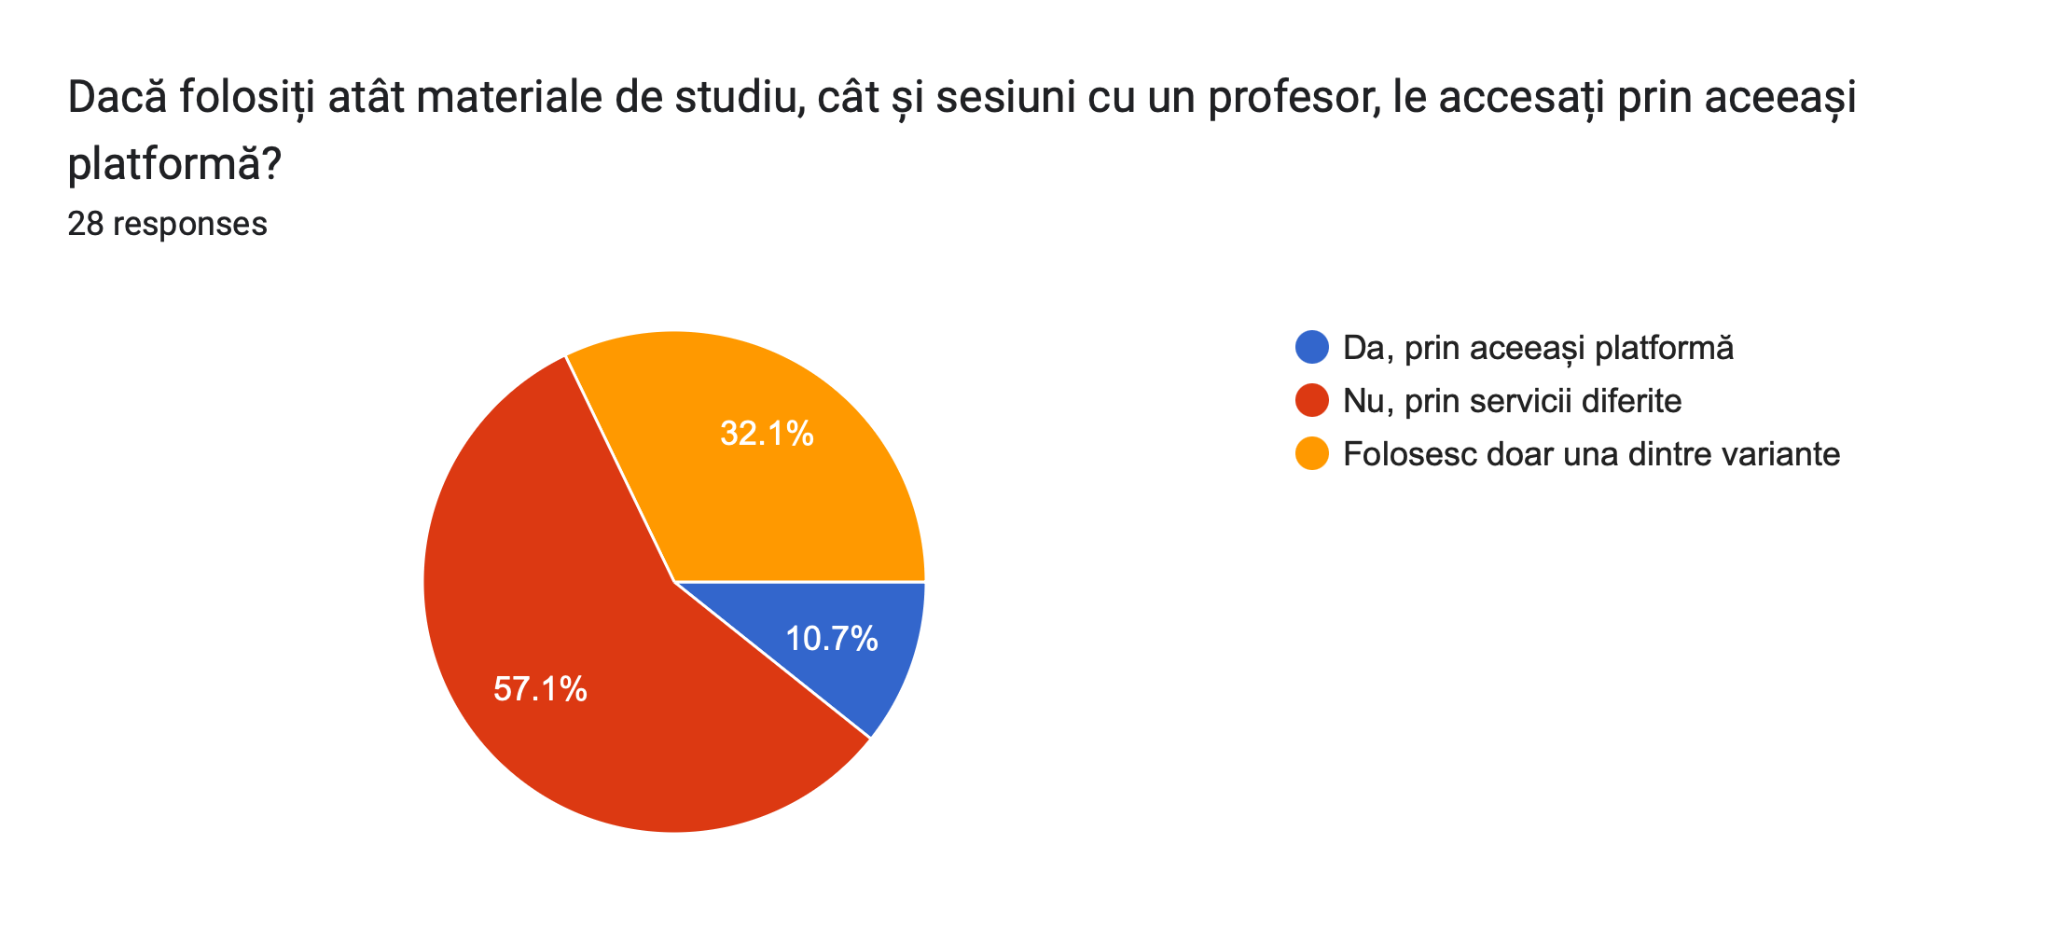
\includegraphics[width=\textwidth]{pics/survey/q04.png}
        \caption{Distribuția modului de acces la materiale de studiu și sesiuni cu un profesor}
        \label{fig:survey-q04}
    \end{subfigure}
    \hfill
    \begin{subfigure}{0.48\textwidth}
        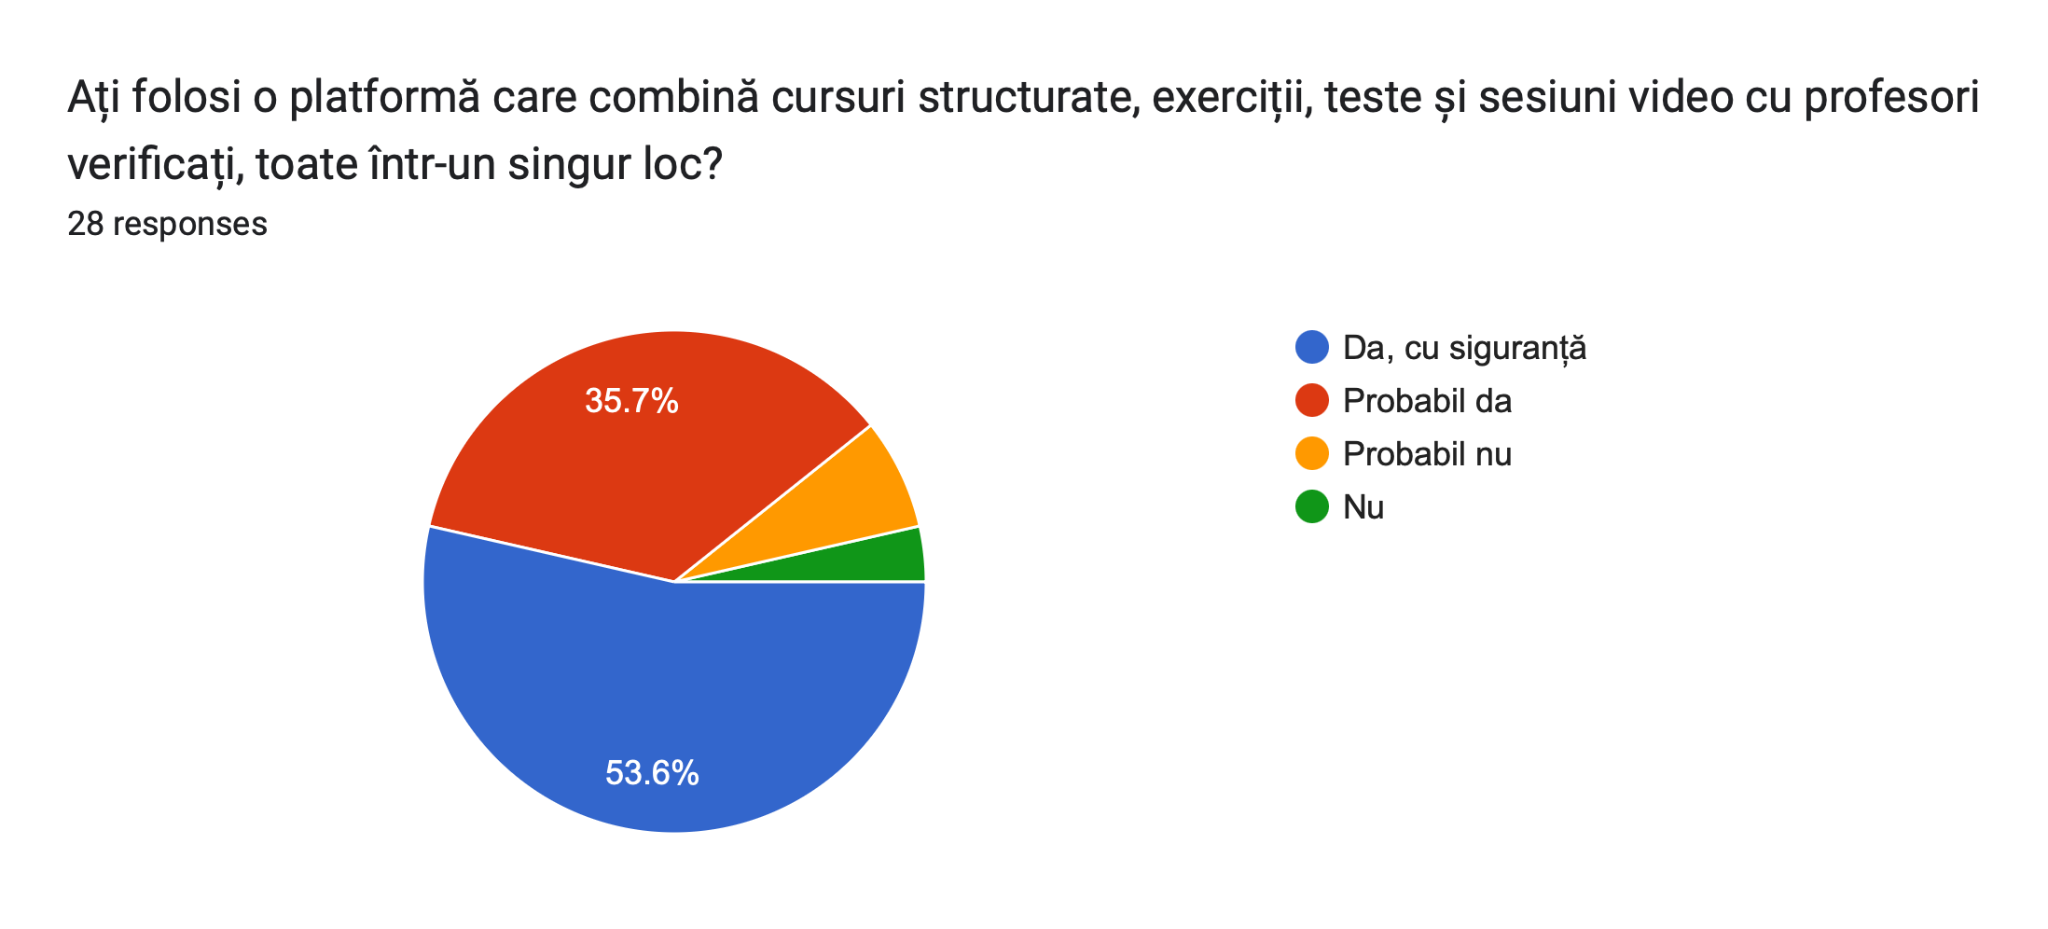
\includegraphics[width=\textwidth]{pics/survey/q07.png}
        \caption{Interesul față de o platformă care integrează materiale de studiu și sesiuni cu profesori}
        \label{fig:survey-q07}
    \end{subfigure}
    \caption{Nevoia de integrare a serviciilor de învățare}
\end{figure}

Nevoia de integrare este susținută și din perspectivă academică, studiul realizat de Tao et al. demonstrând că abordarea combinată, îmbinând studiul individual cu interacțiunea directă cu un profesor, are un impact pozitiv semnificativ asupra competenței în limba engleză față de metodele bazate exclusiv pe studiul individual, studenții care au urmat cursuri bazate pe această abordare înregistrând progrese măsurabile la nivelul tuturor abilităților evaluate \cite{eobtocs_efl_a2024}. Concluzia studiului susține ideea că niciuna dintre cele două componente nu poate asigura singură un progres optim, combinarea lor ducând la rezultate semnificativ mai bune și justificând astfel decizia de a le integra pe ambele într-un singur sistem.

\section{Cerințe de sistem}
Din punctul de vedere al cerințelor de sistem, platforma rulează direct în browser fără a fi necesară instalarea vreunei aplicații separate, singurele condiții tehnice fiind un browser modern și o conexiune stabilă la internet, cerințe pe care orice dispozitiv modern le îndeplinește fără configurări suplimentare.

\section{Categorii de utilizatori}
Platforma este organizată în jurul a trei roluri principale, fiecare cu un set distinct de funcționalități și restricții, accesul la diferite secțiuni ale sistemului fiind condiționat de rolul pe care îl deține utilizatorul și verificat automat la fiecare cerere adresată serverului.

Studentul este utilizatorul principal al platformei, scopul său fiind acela de a studia limba engleză parcurgând materialele disponibile în catalog și interacționând cu profesorii înregistrați în platformă prin sesiuni video, accesul la funcționalitățile platformei fiind condiționat de existența unui cont activ, creat în urma unui proces de verificare prin email. Utilizatorii minori necesită și obținerea consimțământului parental înainte de activarea contului.

Profesorul are un rol dual pe platformă, putând crea conținut educațional și desfășura sesiuni video cu studenții. Accesul la funcționalitățile specifice acestui rol nu este disponibil imediat după înregistrare, ci condiționat de aprobarea unei cereri de activare din partea administratorului, asigurând astfel un nivel minim de verificare a calificărilor înainte de orice interacțiune cu studenții înregistrați.

Administratorul are acces complet la toate entitățile din sistem, rolul său fiind acela de a gestiona utilizatorii, de a valida profesorii și conținutul creat de aceștia și de a menține calitatea generală a platformei, neparticipând el însuși la conținutul didactic, ci coordonând funcționarea întregrului sistem din perspectivă administrativă.

\section{Cerințe funcționale}
Cerințele funcționale ale platformei sunt organizate în jurul celor trei roluri principale și derivă din analiza problemei identificate și din rezultatele sondajului realizat în cadrul proiectului.

\textbf{Cerințele rolului „Student”}

\begin{figure}[htbp]
    \centering
    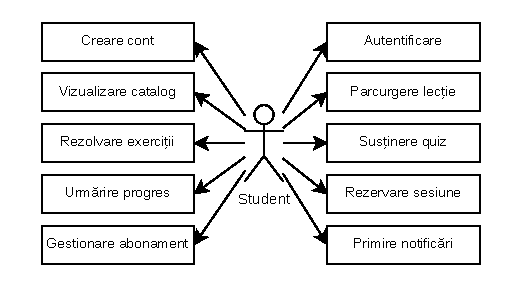
\includegraphics[width=0.8\textwidth]{pics/diagrams/usecase-student.pdf}
    \caption{Diagramă de cazuri de utilizare: Student}
    \label{fig:usecase-student}
\end{figure}

Studentul poate crea un cont completând adresa de email, parola și alte date personale de bază, contul nedevenind activ imediat, ci necesitând confirmarea adresei de email prin accesarea unui link trimis automat de sistem, prevenind astfel înregistrarea cu adrese invalide sau nedeținute de utilizator. În cazul utilizatorilor minori, platforma solicită suplimentar acordul unui părinte sau tutore legal, trimițând o cerere la o adresă de email specificată la înregistrare și activând contul doar după primirea acestui acord, asigurând conformitatea cu cerințele de protecție a datelor pentru persoanele sub 18 ani. Odată autentificat, studentul poate accesa catalogul de cursuri organizate pe trei niveluri de dificultate, parcurgând lecțiile și rezolvând exercițiile interactive asociate fiecăreia, acestea putând fi de mai multe tipuri, incluzând întrebări cu variante de răspuns, completare de spații libere și răspunsuri scurte, fiecare tip de exercițiu evaluând abilități diferite ale studentului.

Marcarea unei lecții ca finalizată este condiționată de rezolvarea corectă a exercițiilor asociate acesteia, platforma asigurându-se astfel că studentul a înțeles conținutul prezentat înainte de a putea avansa, prevenind situația în care acesta ar trece mai departe fără a demonstra că a asimilat informațiile. Pe lângă exerciții, fiecare curs poate conține quiz-uri cronometrate, studentul trebuind să răspundă la toate întrebările în intervalul de timp stabilit de profesor, testul trimițându-se automat la expirarea timpului cu răspunsurile completate până în acel moment. Progresul este urmărit automat la nivel de lecție și de quiz pentru fiecare curs, studentul putând vizualiza oricând câte lecții a finalizat, cate quiz-uri a trecut și un procent general de completare, oferindu-i o imagine clară a evoluției sale fără a fi nevoit să țină singur evidența.

Accesul la sesiunile cu profesori este condiționat de existența unui sold de credite, pe care studentul le poate obține fie printr-un abonament lunar, fie prin achiziționarea lor separată, folosindu-le ulterior pentru rezervări individuale sau de grup în funcție de disponibilitatea profesorilor și de preferința sa, tipul sesiunii influențând numărul de credite deduse. Creditele sunt deduse automat la momentul rezervării, studentul putând consulta oricând istoricul tranzacțiilor și gestiona sau anula abonamentul printr-un portal dedicat, fără a fi necesară intervenția administratorului. De asemenea, studentul primește notificări în aplicație pentru evenimente relevante, cum ar fi confirmarea unei rezervări, remindere înainte de sesiunile programate sau modificări ale conținutului la care are acces (\Cref{fig:usecase-student}).

\textbf{Cerințele rolului „Profesor”}

\begin{figure}[htbp]
    \centering
    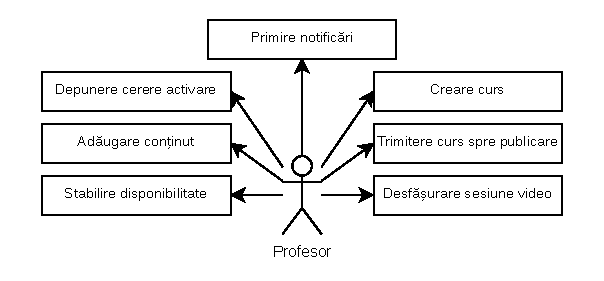
\includegraphics[width=0.8\textwidth]{pics/diagrams/usecase-professor.pdf}
    \caption{Diagramă de cazuri de utilizare: Profesor}
    \label{fig:usecase-professor}
\end{figure}

După crearea contului, profesorul depune o cerere de activare trimisă spre analiză administratorului, neavând acces la funcționalitățile specifice rolului până la aprobare. În cazul respingerii, acesta primește o notificare cu motivul deciziei, putând depunde o nouă cerere după efectuarea modificărilor necesare. Odată aprobat, profesorul poate crea cursuri noi specificând titlul, descrierea și nivelul de dificultate, adăugând lecții cu exerciții interactive de diferite tipuri și quiz-uri cu limită de timp configurabilă, cursurile rămânând în stare de draft până la trimiterea spre publicare și putând fi editate și completate oricând în această perioadă, fără a fi vizibile studenților. La trimiterea spre publicare, cursul intră automat într-un flux de revizuire gestionat de administrator, devenind vizibil în catalog doar după aprobare, profesorul primind o notificare cu decizia luată și, în cazul respingerii, cu observațiile adăugate de administrator.

Profesorul configurează intervalele orare în care este disponibil pentru sesiuni, specificând zilele și orele, sistemul generând automat sloturile disponibile pe baza acestor configurații, ca mai apoi să le afișeze studenților la momentul rezervării, astfel încât aceștia să poată alege un interval potrivit fără a fi nevoie de comunicare directă prealabilă. La momentul sesiunii, profesorul accesează camera video direct din interfața platformei, întreaga interacțiune desfășurându-se fără a fi necesară deschiderea unei aplicații externe, asigurând o experiență unitară în cadrul sistemului. Profesorul este notificat când un student rezervă o sesiune și când administratorul ia o decizie cu privire la un curs trimis spre publicare, putând vedea și eventualele observații adăugate în cazul respingerii, pe care le poate folosi pentru a îmbunătăți conținutul și a-l retrimite (\Cref{fig:usecase-professor}).

\textbf{Cerințele rolului „Administrator”}

\begin{figure}[htbp]
    \centering
    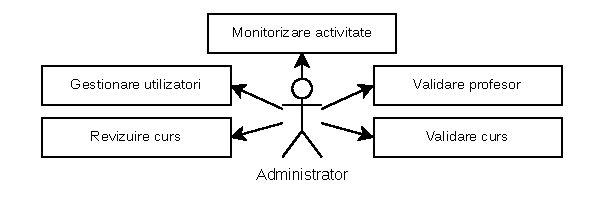
\includegraphics[width=0.8\textwidth]{pics/diagrams/usecase-admin.pdf}
    \caption{Diagramă de cazuri de utilizare: Administrator}
    \label{fig:usecase-admin}
\end{figure}

Administratorul poate vizualiza toți utilizatorii din sistem și poate gestiona conturile acestora, inclusiv să suspende sau să reactiveze un cont în situațiile care impun intervenția sa, având astfel control complet asupra accesului în platformă. Cererile de activare depuse de profesori sunt analizate de administrator, care poate aproba sau respinge fiecare cerere, profesorul primind o notificare automată cu decizia luată și, în cazul respingerii, cu motivul aferent, putând astfel înțelege ce modificări sunt necesare înainte de a depune o nouă cerere. Cursurile trimise de profesori spre publicare intră automat în coada de revizuire a administratorului, care poate aproba publicarea în catalog sau le poate respinge adăugând note cu observațiile sale, vizibile profesorului și utile pentru corectarea conținutului, asigurând astfel că niciun curs nu devine accesibil studenților fără a fi trecut printr-un filtru de calitate. De asemenea, administratorul are acces la o vedere de ansamblu a activității din sistem, putând urmări utilizatorii activi, sesiunile programate și conținutul disponibil în catalog, monitorizând funcționarea generală a platformei (\Cref{fig:usecase-admin}).

\section{Cerințe nefuncționale}
Securitatea reprezintă o cerință esențială, autentificarea utilizatorilor realizându-se prin token-uri cu durată limitată de valabilitate, parolele fiind stocate criptat în baza de date folosind algoritmi de hashing, fără a fi salvate niciodată în format lizibil, eliminând riscul expunerii lor în cazul unui acces neautorizat la baza de date. Accesul la fiecare resursă a sistemului este verificat în funcție de rolul utilizatorului autentificat, un student neputând accesa funcționalitățile unui profesor sau administrator și invers, datele de intrare fiind validate atât în interfața de utilizator, cât și la nivelul serverului, prevenind trimiterea de date invalide sau potențial periculoase.

Performanța platformei trebuie să fie suficient de bună pentru a asigura o experiență fluidă în navigare și în interacțiunea cu conținutul, cererile frecvente cum ar fi încărcarea catalogului sau accesarea unei lecții trebuind să primească răspuns fără întârzieri vizibile, asigurând că utilizatorul nu este nevoit să aștepte la operațiile de bază. Sesiunile video impun o cerință suplimentară de performanță, latența aplicației trebuind să fie suficient de mică pentru a nu afecta calitatea comunicării dintre student și profesor, o conexiune instabilă sau un răspuns lent al serverului putând îngreuna semnificativ interacțiunea. Scalabilitatea este importantă mai ales în contextul unei creșteri a numărului de utilizatori, arhitectura bazată pe token-uri stateless permițând adăugarea de instanțe suplimentare ale serverului fără modificări ale logicii de autentificare, baza de date trebuind să suporte un volum crescut de utilizatori, cursuri și tranzacții fără degradarea timpilor de răspuns.

Interfața trebuie să fie intuitivă și accesibilă indiferent de cât de familiar este utilizatorul cu platformele de e-learning, navigarea între secțiuni trebuind să fie logică și predictibilă pentru toate cele trei roluri, astfel ca fiecare categorie de utilizatori să găsească rapid funcționalitățile de care are nevoie fără a explora extensiv aplicația. Platforma trebuie să funcționeze corect pe browserele moderne uzuale, disponibilitatea sa trebuind să fie ridicată, utilizatorii putând accesa conținutul și rezerva sesiuni oricând fără întreruperi cauzate de probleme tehnice ale sistemului.

\section{Scenarii de utilizare}

\textbf{Scenariul 1: Înregistrarea unui cont de student}

\begin{figure}[htbp]
    \centering
    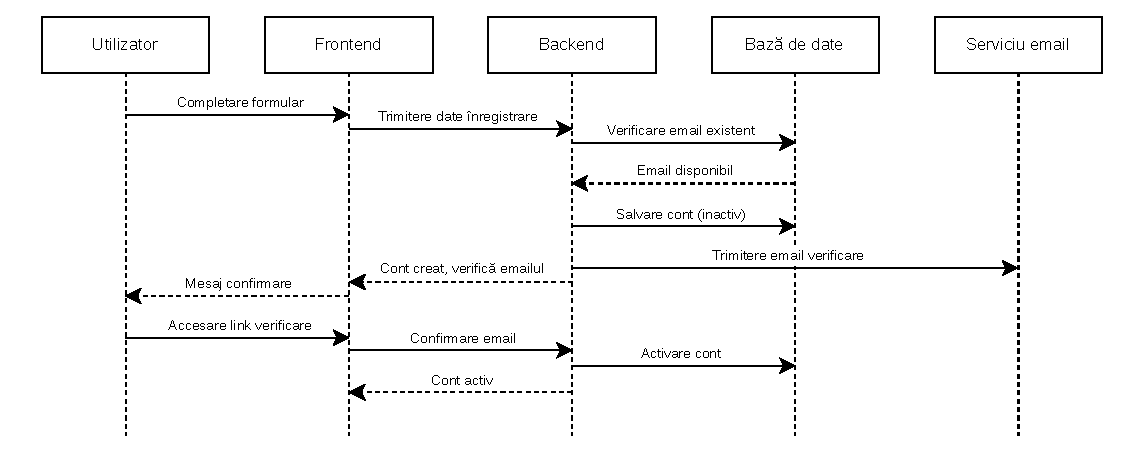
\includegraphics[width=0.8\textwidth]{pics/diagrams/sequence-registration.pdf}
    \caption{Diagramă de secvență: Înregistrarea unui cont de student}
    \label{fig:sequence-registration}
\end{figure}

\textbf{Condiție prealabilă:} utilizatorul nu are un cont existent pe platformă.

Utilizatorul accesează platforma și completează formularul de înregistrare, introducând adresa de email, parola și celelalte date necesare, sistemul validând datele introduse și verificând că adresa de email nu este deja asociată unui cont existent, returnând un mesaj de eroare corespunzător în cazul în care oricare dintre condiții nu este îndeplinită. În cazul utilizatorilor minori, este necesară și obținerea consimțământului parental, platforma trimițând automat o solicitare la adresa de email a părintelui sau tutorelui legal înainte de activarea contului, acesta devenind activ doar după primirea acordului. După validarea cu succes a tuturor datelor, sistemul trimite un email de verificare la adresa introdusă, contul devenind activ doar după confirmarea acestuia prin accesarea link-ului primit, utilizatorul putând apoi accesa toate funcționalitățile disponibile rolului de student și să parcurgă conținutul disponibil în catalog (\Cref{fig:sequence-registration}).

\textbf{Condiție ulterioară:} contul este activ și utilizatorul este autentificat în platformă.

\textbf{Scenariul 2:} Rezervarea unei sesiuni cu un profesor

\begin{figure}[htbp]
    \centering
    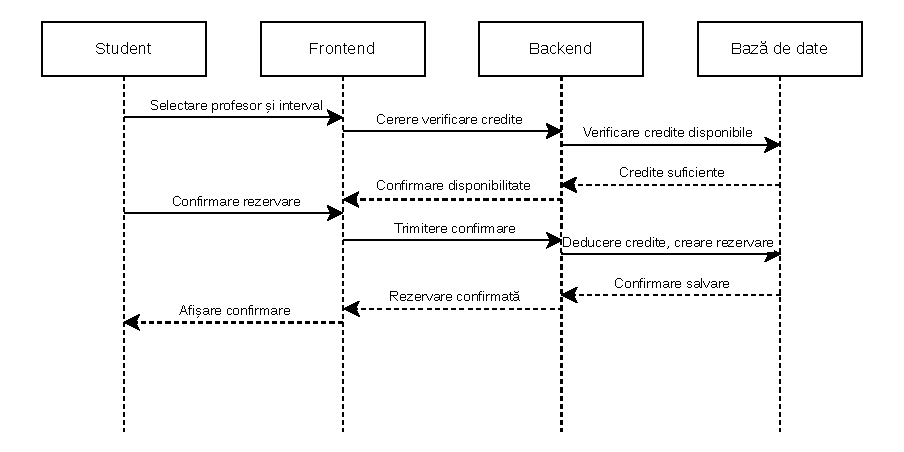
\includegraphics[width=0.8\textwidth]{pics/diagrams/sequence-booking.pdf}
    \caption{Diagramă de secvență: Rezervarea unei sesiuni}
    \label{fig:sequence-booking}
\end{figure}

\textbf{Condiție prealabilă:} studentul are un cont activ și un abonament cu credite disponibile, iar cel puțin un profesor are disponibilitate configurată.

Studentul accesează secțiunea dedicată sesiunilor și vizualizează profesorii disponibili, selectând un profesor și un interval orar din disponibilitatea acestuia, putând alege între o sesiune individuală sau una de grup în funcție de preferință și de oferta disponibilă, fiecare tip de sesiune deducând un număr diferit de credite din contul studentului. Înainte de confirmarea rezervării, sistemul verifică dacă studentul dispune de suficiente credite pentru tipul de sesiune ales. În caz contrar, îi afișează un mesaj corespunzător, nepermițându-i să finalizeze rezervarea fară a dispune de credite suficiente. La confirmarea rezervării, creditele sunt deduse automat din contul studentului, profesorul primind o notificare, iar sesiunea apărând în programul ambilor utilizatori, aceștia putând vedea detaliile complete ale rezervării din profilul lor. La momentul sesiunii, ambii participanți pot accesa camera video direct din interfața platformei, întreaga interacțiune desfășurându-se fără a fi redirecționați către o aplicație externă, asigurând o experiență unitară în cadrul sistemului (\Cref{fig:sequence-booking}).

\textbf{Condiție ulterioară:} sesiunea este rezervată, creditele sunt deduse și sesiunea este vizibilă în contul ambilor utilizatori.

\textbf{Scenariul 3: Crearea și aprobarea unui curs}

\begin{figure}[htbp]
    \centering
    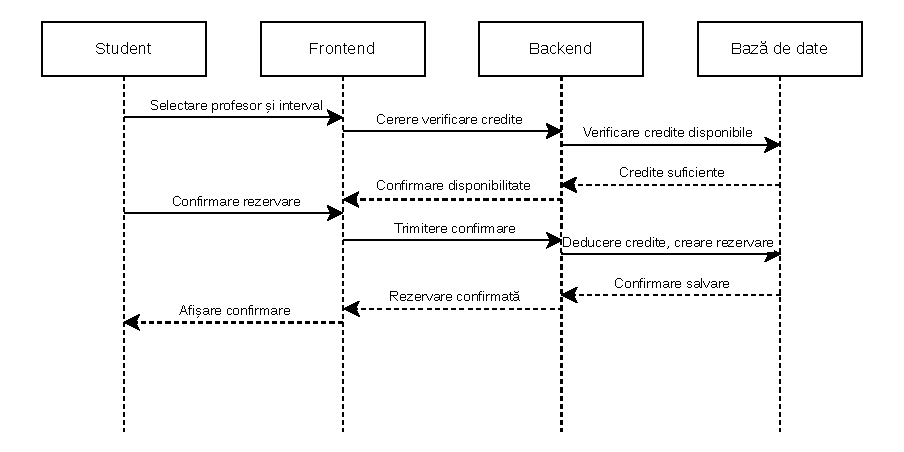
\includegraphics[width=0.8\textwidth]{pics/diagrams/sequence-course-approval.pdf}
    \caption{Diagramă de secvență: Crearea și aprobarea unui curs}
    \label{fig:sequence-course-approval}
\end{figure}

\textbf{Condiție prealabilă:} profesorul are un cont aprobat și activ pe platformă.

Profesorul accesează secțiunea de gestionare a cursurilor și creează un curs nou, completând titlul, descrierea și nivelul de dificultate, adăugând ulterior lecțiile și conținutul asociat fiecăreia, incluzând exerciții interactive de mai multe tipuri și quiz-uri cronometrate, cursul rămânând în stare de draft pe toată durata procesului de creare și putând fi editat oricând, fără a fi vizibil studenților. După finalizare, profesorul trimite cursul spre publicare, acesta intrând automat într-un flux de revizuire gestionat de administrator, care analizează conținutul și poate aproba publicarea în catalog sau poate respinge cursul adăugând note cu motivul deciziei, profesorul primind o notificare cu rezultatul și putând face modificările necesare înainte de a retrimite cursul spre revizuire. Dacă cursul este aprobat, acesta devine imediat vizibil studenților în catalog și poate fi accesat și parcurs, profesorul primind o confirmare a publicării și putând urmări de atunci înainte statistici legate de parcurgerea conținutului de către studenți (\Cref{fig:sequence-course-approval}).

\textbf{Condiție ulterioară:} cursul este publicat în catalog și accesibil studenților sau profesorul este notificat cu privire la respingere și poate efectua modificările necesare.

\chapter{Studiu de piață și metode existente}

\section{Platforme educaționale existente}
Piața platformelor online de învățare a limbilor străine este destul de variată, platformele existente acoperind nevoi diferite ale utilizatorilor și funcționând pe modele de business diferite, fiecare adresând o parte din problemă fără a oferi o soluție completă pentru cineva care vrea atât materiale de studiu structurate, cât și posibilitatea de a lucra direct cu un profesor.

\textbf{Duolingo}

Duolingo este probabil cea mai cunoscută platformă de învățare a limbilor străine la nivel global, punând la dispoziția utilizatorilor lecții scurte bazate pe mecanisme de tip joc, organizate pe niveluri de dificultate și accesibile gratuit în varianta de bază, cu o versiune premium care adaugă funcționalități suplimentare și elimină reclamele, modelul platformei bazându-se pe încurajarea unui obicei zilnic de studiu prin recompense și streak-uri \cite{duolingo}. Această abordare o face potrivită pentru utilizatorii care vor să studieze câteva minute pe zi fără un angajament serios față de un program de studiu, platforma reușind să atragă un număr foarte mare de utilizatori tocmai prin accesibilitatea și simplitatea experienței pe care o oferă.

Limitele devin evidente atunci când utilizatorul dorește mai mult decât exerciții scurte și recompense virtuale, platforma neoferind niciun mecanism de interacțiune cu un profesor real, conținutul fiind standardizat și identic pentru toți utilizatorii fără a putea fi adaptat nevoilor individuale, iar sistemul de urmărire a progresului bazându-se pe indicatori gamificați care nu reflectă neapărat un nivel lingvistic real și funcțional.

\textbf{Coursera}

Coursera funcționează pe un model complet diferit față de Duolingo, punând accentul pe cursuri academice create de universități și instituții de prestigiu din întreaga lume, organizate în module cu materiale video, teme și evaluări, finalizarea unui curs ducând la obținerea unui certificat recunoscut care poate fi adăugat în CV-ul profesional al utilizatorului \cite{coursera}. Nivelul conținutului disponibil pe platformă este ridicat, Coursera adresându-se în principal utilizatorilor care vor să urmeze un curs structurat serios, nu neapărat să practice engleza conversațional sau să primească îndrumare personalizată din partea unui profesor.

Interacțiunea directă cu un profesor lipsește complet din modelul standard al platformei, comunicarea limitându-se la forumuri de discuții unde studenții interacționează între ei sau cu asistenți de curs, sesiunile live nefiind parte din oferta obișnuită, conținutul fiind preînregistrat și identic pentru toți utilizatorii indiferent de nivelul sau obiectivele lor specifice.

\textbf{iTalki}

iTalki funcționează ca o piață de meditații online, conectând studenți cu profesori sau vorbitori nativi disponibili pentru sesiuni individuale tarifate per sesiune, oferind o gamă largă de profesori pentru aproape orice limbă la prețuri foarte variate, ceea ce o face accesibilă financiar pentru mulți utilizatori \cite{italki}. Flexibilitatea este principalul avantaj al platformei, studenții putând alege profesori în funcție de preț, disponibilitate și recenziile primite de la alți utilizatori.

Problema principală a iTalki constă în faptul că nu oferă niciun plan de studiu propriu sau structurare a procesului de învățare, fiecare sesiune fiind practic independentă de celelalte, profesorul neavând acces la niciun fel de informație despre ce a studiat studentul până în acel moment și neputând adapta sesiunea în funcție de lacunele sau obiectivele specifice ale acestuia. În plus, lipsa unui proces formal de verificare a calificărilor profesorilor face ca oricine să poată crea un profil și oferi sesiuni, calitatea variind astfel considerabil de la un profesor la altul și lăsând studentul să evalueze singur dacă alegerea sa a fost bună.

\textbf{Preply}

Preply funcționează pe un model similar cu iTalki, conectând studenți cu profesori pentru sesiuni online individuale, dar adăugând față de aceasta un strat suplimentar de structurare, incluzând unele materiale de studiu integrate în platformă și un proces de selecție mai riguros pentru profesori, ceea ce o face o alegere mai sigură pentru utilizatorii care vor să lucreze cu cineva verificat \cite{preply}. Platforma urmărește și progresul studentului la nivel de sesiuni susținute, oferind o imagine mai clară a activității față de alte platforme de meditații online.

Chiar și cu aceste îmbunătățiri față de iTalki, materialele de studiu disponibile de Preply nu sunt integrate organic cu sesiunile live, rămânând mai degrabă resurse auxiliare decât un plan de studiu coerent urmărit sistematic împreună cu profesorul, iar progresul urmărit reflectând în principal numărul de sesiuni susținute, nu competențele efectiv dobândite prin parcurgerea unui conținut structurat. Din toate platformele analizate, Preply este cea mai apropiată de conceptul platformei propuse în această lucrare, dar distanța dintre ele rămâne semnificativă în ceea ce privește integrarea conținutului didactic cu sesiunile video.

\section{Analiză comparativă a platformelor}

Din analiza celor patru platforme se conturează clar o separare între cele două segmente identificate în capitolul 2, platformele de conținut neoferind interacțiune directă cu profesori, iar platformele de meditații online neavând un plan de studiu propriu integrat, niciuna dintre ele acoperind complet nevoile unui utilizator care dorește ambele lucruri din același loc.

\Cref{tab:platform-comparison} centralizează compararea celor patru platforme pe criteriile esențiale care asigură o experiență completă de învățare a limbii engleze, evidențiind golul pe care platforma propusă în această lucrare încearcă să îl acopere.

\begin{table}[htbp]
    \centering
    \resizebox{\textwidth}{!}{%
        \begin{tabular}{l c c c c}
            \toprule
            \textbf{Criteriu} & \textbf{Duolingo} & \textbf{Coursera} & \textbf{iTalki} & \textbf{Preply} \\
            \midrule
            Materiale de studiu structurate & Da & Da & Nu & Parțial \\
            Sesiuni video cu profesori & Nu & Nu & Da & Da \\
            Urmărire progres & Da & Da & Nu & Parțial \\
            Verificare profesori & Nu & Nu & Parțial & Da \\
            Model de plată & Gratuit/Premium & Abonament/Per curs & Per sesiune & Abonament \\
            \bottomrule
        \end{tabular}%
    }
    \caption{Analiza comparativă a platformelor educaționale existente}
    \label{tab:platform-comparison}
\end{table}

\section{Tehnologii utilizate și alternative}
Alegerea tehnologiilor pentru implementarea platformei a urmărit în principal potrivirea cu cerințele funcționale identificate și compatibilitatea componentelor între ele, fiecare decizie fiind luată după analizarea alternativelor disponibile și argumentată atât din punct de vedere calitativ, cât și cantitativ acolo unde a fost posibil.

\subsection{Frontend}
Pentru interfața de utilizator a fost ales Next.js, un framework bazat pe React, care îi extinde funcționalitățile de bază cu suport nativ pentru randare pe server, generare statică a paginilor și un sistem de rutare bazat pe structura de fișiere a proiectului, reducând semnificativ configurarea necesară față de o aplicație React obișnuită și oferind performanță mai bună la prima încărcare a paginilor \cite{nextjs}. Alegerea Next.js față de React a venit din nevoia de randare pe server a paginilor publice ale platformei, îmbunătățind experiența utilizatorului și comportamentul general al aplicației fără a sacrifica interactivitatea necesară secțiunilor dinamice.

Alternativa principală luată în considerare a fost Nuxt.js, meta-framework-ul construit peste Vue.js care oferă suport nativ pentru randare pe server, similar cu ce oferă Next.js pentru React, beneficiind de o curbă de învățare mai ușoară și o sintaxă considerată mai accesibilă față de React \cite{nuxtjs}. Decizia de a nu folosi Nuxt.js a venit din faptul că ecosistemul de biblioteci disponibil pentru React și Next.js este considerabil mai bogat, oferind mai multe opțiuni pentru funcționalitățile necesare platformei (\Cref{tab:frontend-comparison}).

\begin{table}[htbp]
    \centering
    \small
    \begin{tabular}{l c c}
        \toprule
        \textbf{Criteriu} & \textbf{Next.js} & \textbf{Nuxt.js} \\
        \midrule
        Randare pe server & Da & Da \\
        Limbaj principal & JavaScript/TypeScript & JavaScript/TypeScript \\
        Curbă de învățare & Medie & Mică \\
        Ecosistem biblioteci & Foarte mare & Mediu \\
        Rutare integrată & Da & Da \\
        \bottomrule
    \end{tabular}
    \caption{Compararea framework-urilor frontend}
    \label{tab:frontend-comparison}
\end{table}

\subsection{Backend}
Pentru server a fost ales Spring Boot, un framework bazat pe Java care simplifică configurarea aplicațiilor Spring, oferind funcționalități integrate pentru construirea de REST API-uri, gestionarea securității prin Spring Security și accesul la baza de date prin JPA, impunând totodată o structură clară a codului care face aplicația mai ușor de întreținut și de extins pe termen lung \cite{springboot}. Alegerea Spring Boot a venit în principal din nevoia de a gestiona funcționalități complexe ale aplicației, care implică roluri și permisiuni, fluxuri de aprobare, sisteme de credite și integrări cu servicii externe, toate acestea beneficiind de structura și instrumentele pe care le oferă ecosistemul Spring.

Principala alternativă considerată a fost Express.js, un framework minimalist pentru Node.js bazat pe JavaScript, apreciat pentru flexibilitatea sa și pentru rapiditatea cu care poate fi pornit un server funcțional, bazându-se pe un model asincron care îl face eficient pentru operații de tip I/O și potrivit pentru API-uri simple cu cerințe mai puțin complexe \cite{expressjs}. Lipsa unei structuri impuse poate fi un avantaj pentru proiecte mici, dar devine un dezavantaj pe măsură ce aplicația crește, codul riscând să devină greu de urmărit și de întreținut, iar absența unui sistem de securitate integrat comparabil cu Spring Security reprezentând un argument suplimentar în favoarea alegerii Spring Boot pentru nevoile acestei platforme (\Cref{tab:backend-comparison}).

\begin{table}[htbp]
    \centering
    \small
    \begin{tabular}{l c c}
        \toprule
        \textbf{Criteriu} & \textbf{Spring Boot} & \textbf{Express.js} \\
        \midrule
        Limbaj & Java & JavaScript/TypeScript \\
        Securitate integrată & Da & Nu \\
        Structură impusă & Da & Nu \\
        Model execuție & Multi-thread & Single-thread asincron \\
        Complexitate configurare & Medie & Mică \\
        \bottomrule
    \end{tabular}
    \caption{Compararea framework-urilor backend}
    \label{tab:backend-comparison}
\end{table}

\subsection{Bază de date}
Pentru stocarea datelor a fost aleasă PostgreSQL, o bază de date relațională open source cu suport pentru tranzacții complexe, integritate referențială și un limbaj SQL extins cu funcționalități avansate, alegerea unui model relațional venind firesc din structura datelor platformei, entitățile sistemului formând relații clare și bine definite între ele: utilizatorii, cursurile, lecțiile, sesiunile și tranzacțiile se leagă unele de altele în mod natural într-o schemă relațională \cite{postgresql}.

Alternativa analizată a fost MongoDB, o bază de date de tip NoSQL orientată pe documente cu o schemă flexibilă care permite câmpuri diferite de la un document la altul, funcționând bine pentru date nestructurate sau cu schemă variabilă și oferind o scalabilitate orizontală mai ușor de realizat față de bazele de date relaționale tradiționale \cite{mongodb}. Pentru platforma propusă, datele au o structură fixă și bine definită, iar operații precum deducerea creditelor la momentul rezervării necesită consistența și integritatea datelor pe care PostgreSQL le asigură nativ, MongoDB nefiind la fel de potrivit pentru acest tip de cerințe (\Cref{tab:database-comparison}).

\begin{table}[htbp]
    \centering
    \small
    \begin{tabular}{l c c}
        \toprule
        \textbf{Criteriu} & \textbf{PostgreSQL} & \textbf{MongoDB} \\
        \midrule
        Tip & Relațional & Non-relațional \\
        Schemă & Fixă & Flexibilă \\
        Relații complexe & Da & Limitat \\
        Consistență tranzacțională & Da & Parțial \\
        Open Source & Da & Da \\
        \bottomrule
    \end{tabular}
    \caption{Compararea soluțiilor de stocare a datelor}
    \label{tab:database-comparison}
\end{table}

\subsection{Integrări externe}
Pe lângă tehnologiile principale utilizate, platforma integrează trei servicii externe pentru funcționalități care ar fi necesitat un efort semnificativ de implementare de la zero și care sunt mai bine gestionate prin servicii specializate.

Sesiunile video sunt gestionate prin Daily.co, un serviciu care oferă o infrastructură completă de videoconferință accesibilă prin API, permițând crearea de camere de sesiune și desfășurarea apelurilor video direct în browser, fără ca utilizatorul să fie nevoit să instaleze o aplicație separată, întreaga interacțiune desfășurându-se în cadrul platformei \cite{dailyco}. Chiar dacă serviciile similare de videoconferință disponibile pe piață aveau funcționalități similare, Daily.co s-a diferențiat prin simplitatea integrării și prin faptul că oferă o interfață video completă care poate fi inclusă direct în aplicație, reducând semnificativ timpul de implementare.

Sistemul de plăți și abonamente este gestionat prin Stripe, un serviciu de procesare a plăților online cu suport pentru abonamente recurente, webhook-uri pentru notificarea serverului la evenimentele de plată și un portal dedicat prin care utilizatorii își pot gestiona singuri abonamentul fără a fi necesară intervenția unui administrator \cite{stripe}. Spre deosebire de celelalte soluții de procesare a plăților, Stripe oferă o documentație mai bine structurată, un API mai modern și un set complet de funcționalități pentru gestionarea abonamentelor, reprezentând astfel alegerea mai potrivită pentru nevoile platformei.

Migrările bazei de date sunt gestionate prin Flyway, un instrument care versionează modificările aduse structurii bazei de date prin fișiere SQL numerotate aplicate automat la pornirea aplicației, asigurând astfel că schema bazei de date este întotdeauna la versiunea corectă și că nicio migrare nu este aplicată de mai multe ori \cite{flyway}. Față de alte instrumente similare de versionare a schemei bazei de date, Flyway a fost preferat datorită simplității și integrării native cu Spring Boot, necesitând configurare minimă pentru a funcționa corect.

\chapter{Soluția propusă}

\section{Arhitectura generală a sistemului}
Platforma este construită pe o arhitectură de tip client-server, în care interfața de utilizator și logica serverului sunt separate și comunică exclusiv prin intermediul unui REST API, fiecare componentă putând fi dezvoltată și întreținută independent de cealaltă. \Cref{fig:system-architecture} prezintă o vedere de ansamblu a sistemului, arătând componentele principale și relațiile dintre ele.

\begin{figure}[htbp]
    \centering
    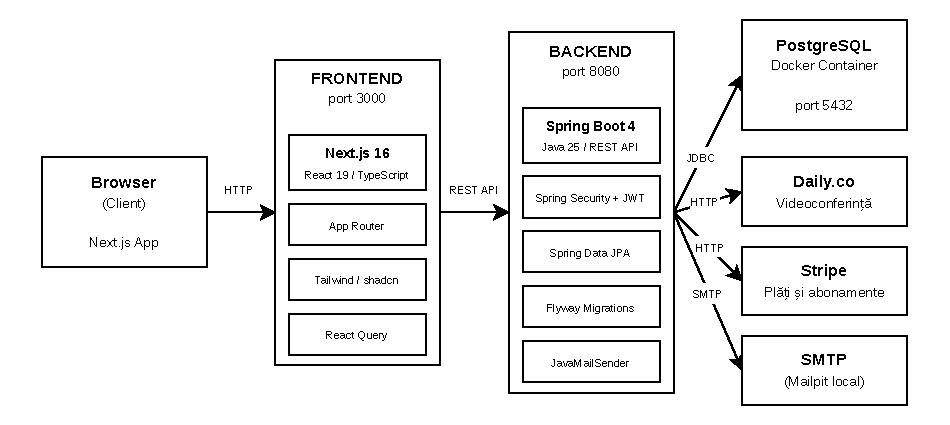
\includegraphics[width=0.8\textwidth]{pics/diagrams/system-architecture.pdf}
    \caption{Arhitectura generală a sistemului}
    \label{fig:system-architecture}
\end{figure}

Componenta client este o aplicație Next.js care rulează în browserul utilizatorului, trimițând cereri HTTP către server și afișând datele primite ca răspuns, fără a deține logica din spatele aplicației sau acces direct la baza de date. Componenta server este o aplicație Spring Boot care expune un REST API, ce procesează cererile primite de la client, aplică regulile aplicației și interacționează cu baza de date și cu serviciile externe, returnând răspunsuri în format JSON. Practic, clientul nu știe cum funcționează serverul și invers, cei doi comunicând doar prin cereri și răspunsuri HTTP bine definite.

Autentificarea se realizează prin token-uri JWT, clientul primind un token la autentificare și incluzându-l în headerul fiecărei cereri ulterioare \cite{jwt}. Serverul verifică validitatea acestuia și extrage identitatea și rolul utilizatorului înainte de a procesa cererea, returnând un răspuns cu codul 401 dacă token-ul lipsește sau nu este valid. Abordarea aceasta face serverul stateless, nefiind nevoie să stocheze sesiuni active ale utilizatorilor.

Baza de date PostgreSQL rulează într-un container Docker separat, serverul conectându-se la aceasta prin JDBC, iar schema bazei de date este gestionată și versionată prin Flyway, care aplică automat migrările SQL la pornirea aplicației.

Serviciile externe, Daily.co pentru sesiunile video, Stripe pentru plăți și abonamente și serverul SMTP pentru emailuri, sunt accesate exclusiv de server prin cereri HTTP, clientul neavând niciun contact direct cu acestea.

\section{Modelul bazei de date}
Baza de date este organizată în mai multe grupuri de tabele, fiecare acoperind un domeniu funcțional distinct al sistemului, toate conectate prin foreign keys care asigură integritatea datelor. Diagrama entitate-relație completă a bazei de date este prezentată în Anexa B (\Cref{fig:er-diagram}).

Primul grup acoperă gestionarea utilizatorilor, tabela \texttt{users} stocând informațiile de bază ale fiecărui utilizator, inclusiv rolul în sistem și statusul contului, ambele câmpuri fiind verificate de server la fiecare cerere autentificată. Al doilea grup acoperă conținutul didactic, cursurile, lecțiile, exercițiile și quiz-urile, formând o ierarhie clară în care fiecare entitate are câmpuri dedicate pentru statusul de publicare și, în cazul cursurilor, pentru statusul de revizuire, controlând ce este vizibil studenților și ce se află în așteptarea aprobării.

Progresul studenților este urmărit prin tabele separate, una pentru progresul la nivel de lecție și alta pentru sesiunile de quiz. Tabela \texttt{quiz\_attempts} stochează răspunsurile date la fiecare întrebare împreună cu momentul de start al sesiunii, permițând serverului să verifice dacă limita de timp a fost respectată la momentul trimiterii.

Sesiunile video sunt reprezentate prin tabela \texttt{meetings}, fiecare sesiune având asociat un profesor, un interval orar planificat și un identificator al camerei din Daily.co, participanții și statusul lor individual (rezervat, prezent sau absent), fiind stocate într-o tabelă separată. Disponibilitatea profesorilor este configurată prin intervale orare recurente săptămânale, pe baza cărora serverul calculează automat sloturile disponibile ținând cont de sesiunile deja rezervate.

Sistemul de facturare folosește mai multe tabele interconectate, abonamentele stocând informațiile despre planul activ al fiecărui student și datele de reînnoire primite de la Stripe, balanța de credite fiind gestionată separat printr-un mecanism care previne deducerea incorectă a creditelor în cazul rezervărilor simultane. Un jurnal de tranzacții înregistrează fiecare modificare a balanței cu motivul aferent, oferind o imagine completă a istoricului de credite.

\section{Componenta client}
Componenta client este dezvoltată în Next.js, folosind App Router, sistemul de rutare bazat pe structura directorului \texttt{app}, în care fiecare director corespunde unei rute sau unui grup de rute cu comportament comun (\Cref{fig:client-structure}).

Structura paginilor este organizată pe niveluri de acces: paginile publice accesibile fără autentificare, paginile disponibile oricărui utilizator autentificat și paginile specifice fiecărui rol. Accesul este verificat la nivelul fiecărei componente, utilizatorul neautorizat fiind redirecționat automat. Paginile specifice profesorului acoperă crearea și gestionarea cursurilor și configurarea disponibilității, în timp ce paginile administratorului acoperă gestionarea utilizatorilor, aprobarea profesorilor și revizuirea cursurilor.

Comunicarea cu serverul este gestionată prin TanStack Query, cunoscut anterior ca React Query, care se ocupă automat de cache-ul datelor, invalidând cache-ul la operații de scriere și reîncărcând informațiile afectate fără a fi nevoie de cod suplimentar \cite{reactquery}. De exemplu, după rezervarea unei sesiuni, lista sesiunilor și balanța de credite se actualizează automat în interfață.

Starea de autentificare a utilizatorului este menținută pe tot parcursul sesiunii și sincronizată între tab-uri. Un utilizator care se deconectează dintr-un tab poate vedea modificarea reflectată automat în toate celelalte tab-uri deschise, fără a fi necesar ca acesta să reîncarce pagina sau să facă altă acțiune.

Pentru interfața vizuală s-au folosit Tailwind CSS și componente din shadcn/ui, primul oferind un sistem de clase care permite stilizarea directă în markup, iar al doilea furnizând componente accesibile și ușor de personalizat care asigură o experiență vizuală consistentă pe întreaga platformă \cite{tailwind}\cite{shadcn}. Aplicația funcționează corect pe orice dimensiune de ecran, layout-ul adaptându-se automat atât pentru desktop, cât și pentru dispozitive mobile, fără a fi nevoie de o versiune separată pentru fiecare.

\begin{figure}[htbp]
    \centering
    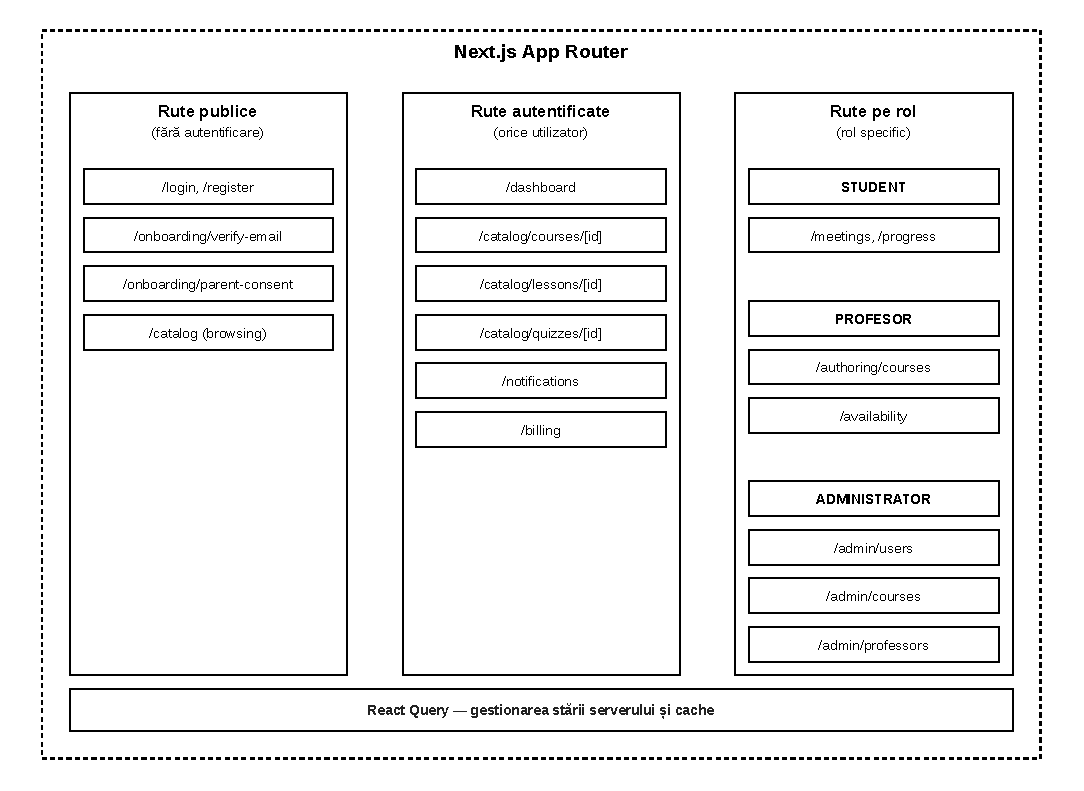
\includegraphics[width=0.8\textwidth]{pics/diagrams/client-structure.pdf}
    \caption{Structura componentei client}
    \label{fig:client-structure}
\end{figure}

\section{Componenta server}
Componenta server este organizată în trei straturi principale cu responsabilități clare, comunicând între ele într-o singură direcție, de la controller spre repository. \Cref{fig:server-layers} prezintă această structură.

Stratul „controller” gestionează cererile HTTP primite de la client, fiecare controller acoperind un domeniu funcțional specific, autorizarea realizându-se prin adnotarea \texttt{@PreAuthorize} care verifică rolul utilizatorului înainte de a permite accesul la o metodă. Validarea datelor trimise de client se face tot la acest nivel, serverul returnând automat un răspuns cu codul 400 și detaliile erorii dacă datele nu respectă constrângerile definite.

Stratul „service” conține logica aplicației și coordonează operațiile între mai multe repository-uri atunci când este necesar. La rezervarea unei sesiuni, de exemplu, serviciul verifică disponibilitatea profesorului, numărul creditelor studentului și absența conflictelor, toate acestea înainte de a crea o intrare în baza de date și a deduce creditele. Tranzacțiile bazei de date sunt gestionate la acest nivel, operațiile care implică mai multe modificări grupându-se într-o singură tranzacție pentru a asigura că fie toate reușesc, fie niciuna nu este aplicată.

Stratul „repository” asigură accesul la baza de date prin Spring Data JPA, expunând operații standard și metode personalizate generate automat pe baza numelui metodei sau definite explicit prin adnotarea \texttt{@Query} pentru interogări mai complexe.

Securitatea serverului este asigurată prin Spring Security, configurat să intercepteze toate cererile primite, să extragă și să valideze token-ul JWT din header și să populeze contextul de securitate cu identitatea utilizatorului, permițând astfel ca adnotările \texttt{@PreAuthorize} să funcționeze corect.

\begin{figure}[htbp]
    \centering
    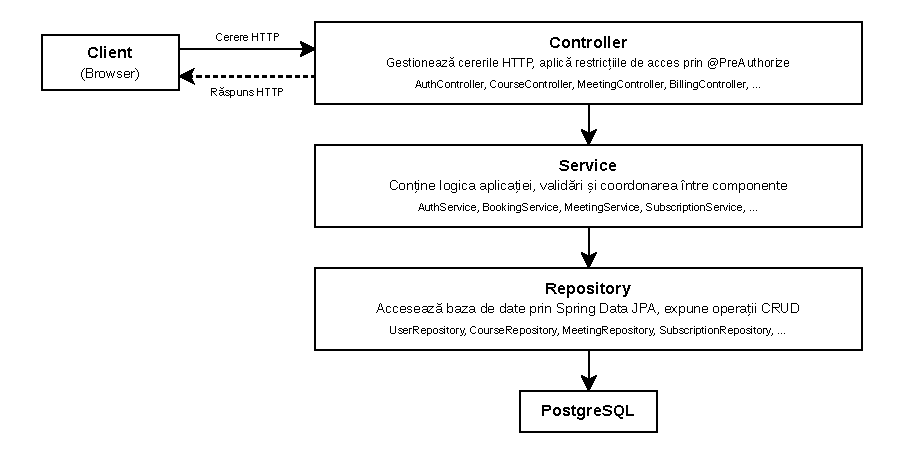
\includegraphics[width=0.8\textwidth]{pics/diagrams/server-layers.pdf}
    \caption{Structura componentei server}
    \label{fig:server-layers}
\end{figure}

\section{Integrări externe}
Platforma integrează trei servicii externe pentru funcționalități specializate care ar fi necesitat un efort semnificativ de implementare de la zero.

Integrarea cu Daily.co gestionează ciclul de viața al camerelor de sesiune video. Serverul creează programatic o cameră la momentul rezervării și furnizează clientului token-ul de acces necesar pentru a intra în cameră direct din interfața platformei, fără a fi redirecționat în altă aplicație. Tot ce știe clientul despre sesiunea video este un URL și un token, restul comunicării cu Daily.co realizându-se exclusiv pe server. La anularea sau finalizarea unei sesiuni, camera este ștearsă automat pentru a nu acumula resurse neutilizate.

Integrarea cu Stripe acoperă întregul flux de facturare, de la crearea unui abonament și procesarea primei plăți până la reînnoirile recurente și anulările. Serverul primește notificări despre evenimentele de plată prin webhook-uri și actualizează statusul abonamentului și balanța de credite a studentului în consecință, idempotența procesării fiind asigurată prin stocarea identificatorului fiecărui eveniment procesat pentru a evita procesarea duplicatelor. Studentul poate gestiona singur abonamentul printr-un portal Stripe accesat direct din platformă.

Integrarea cu serverul SMTP este folosită pentru trimiterea emailurilor de verificare la înregistrare, a solicitărilor de consimțământ parental pentru utilizatorii minori și a notificărilor despre deciziile administratorului, emailurile fiind trimise asincron pentru a nu bloca procesarea celorlalte cereri.

\chapter{Detalii de implementare}

\section{Autentificare și securitate}
Autentificarea utilizatorilor este implementată prin token-uri JWT, fiecare utilizator primind un token de acces la autentificarea cu succes, pe care îl include în headerul \texttt{Authorization} al fiecărei cereri ulterioare adresate serverului. Token-ul conține în payload identitatea utilizatorului și rolul acestuia, serverul putând extrage aceste informații direct din token fără a interoga baza de date la fiecare cerere, ceea ce reduce semnificativ numărul de operații de citire necesare pentru procesarea cererilor autentificate. Token-urile au o durată de valabilitate limitată care, după expirare, obligă utilizatorul să se autentifice din nou pentru a obține un token nou.

Spring Security este configurat să intercepteze toate cererile primite înainte de a ajunge la controller, un filtru dedicat extrăgând token-ul din header, validând semnătura și termenul de valabilitate și populând contextul de securitate cu identitatea utilizatorului. Dacă token-ul lipsește sau nu este valid, cererea este respinsă imediat cu codul 401, fără a mai ajunge la controller.

Parolele utilizatorilor nu sunt stocate în format text în baza de date. Înainte de salvare, fiecare parolă este trecută printr-un algoritm de hashing BCrypt, autentificarea verificând ulterior dacă hash-ul parolei introduse corespunde celui stocat, fără a exista vreodată posibilitatea de a recupera parola originală din baza de date.

Procesul de înregistrare a presupus câteva decizii mai puțin evidente legate de activarea contului. Un cont nou creat rămâne inactiv până la verificarea adresei de email, serverul generând un token unic de verificare trimis automat la adresa specificată la înregistrare, contul activându-se la accesarea linkului care conține token-ul. Pentru utilizatorii minori există un pas suplimentar față de verificarea obișnuită a emailului, platforma solicitând și consimțământul unui părinte sau tutore legal prin trimiterea unui link separat la o adresă specificată la înregistrare, contul rămânând inactiv până la confirmarea din ambele părți. Asta a necesitat gestionarea unor stări intermediare ale contului și verificarea la autentificare că toate etapele de activare au fost finalizate înainte de a permite accesul în platformă (\Cref{fig:login}).

Autorizarea la nivel de endpoint este implementată prin adnotarea \texttt{@PreAuthorize} pe metodele controller-ului, fiecare metodă specificând ce rol trebuie să aibă utilizatorul autentificat pentru a putea apela endpoint-ul respectiv. Un student nu poate accesa funcționalitățile unui profesor chiar dacă cunoaște URL-ul exact al endpoint-ului, serverul respingând cererea cu codul 403 înainte de a executa orice logică (\Cref{fig:security-filter-chain}).

\section{Gestionarea cursurilor și fluxul de aprobare}
Cursurile trec printr-un ciclu de viață definit de la creare până la publicare, statusul unui curs controlând vizibilitatea sa și operațiile permise asupra lui la fiecare moment. Un curs nou are statusul \texttt{DRAFT} și nu este vizibil studenților, profesorul putând edita titlul, descrierea, nivelul de dificultate și tot conținutul din interiorul cursului cât timp acesta se află în această stare. La trimiterea spre publicare, statusul trece în \texttt{IN\_REVIEW}, cursul devenind vizibil administratorului în coada de revizuire, dar în continuare invizibil studenților (\Cref{fig:course-approval}).

Administratorul poate aproba sau respinge cursul. La aprobare statusul devine \texttt{PUBLISHED} și cursul apare imediat în catalog, profesorul primind o notificare automată cu decizia. La respingere statusul revine la \texttt{DRAFT} și profesorul primește o notificare însoțită de observațiile administratorului, putând face modificările necesare și retrimite spre publicare. Practic, un curs poate trece de mai multe ori prin ciclul \texttt{DRAFT} $\rightarrow$ \texttt{IN\_REVIEW} $\rightarrow$ \texttt{DRAFT} înainte de a fi aprobat.

Lecțiile și exercițiile din interiorul unui curs au propriul status de publicare, independent de cel al cursului, ceea ce înseamnă că un profesor poate publica un curs cu doar o parte din lecții vizibile, adăugându-le pe restul ulterior fără a scoate cursul din catalog. Asta a adăugat complexitate interogărilor serverului, care trebuie să filtreze conținutul după mai multe niveluri de status simultan când un student accesează un curs.

Un aspect important al fluxului de aprobare este că un profesor nu poate modifica un curs aflat în \texttt{IN\_REVIEW}, statusul blocând editarea până când administratorul ia o decizie. Această restricție a fost introdusă pentru a evita situația în care profesorul modifică conținutul în timp ce administratorul îl revizuiește, ceea ce ar putea face ca decizia administratorului să nu mai reflecte versiunea curentă a cursului (\Cref{fig:course-review-transitions}).

\section{Sistemul de rezervare a sesiunilor}
Disponibilitatea profesorilor este configurată prin intervale orare recurente săptămânale, fiecare interval specificând ziua săptămânii, ora de start și durata. Pe baza acestor intervale, serverul calculează dinamic sloturile disponibile pentru o perioadă de timp, excluzându-le automat pe cele deja rezervate sau care se suprapun cu alte sesiuni existente. Sloturile nu sunt precalculate și stocate în baza de date, ci generate la cerere, ceea ce înseamnă că disponibilitatea afișată studentului reflectă întotdeauna situația curentă fără riscul de a afișa sloturi expirate (\Cref{fig:availability}).

Procesul de rezervare implică mai mulți pași de validare executați în cadrul aceleiași tranzacții. Serverul verifică că intervalul orar selectat este înca liber, că studentul are suficiente credite pentru tipul de sesiune ales, individual sau de grup, și că nu există o altă rezervare a aceluiași student care se suprapune cu intervalul selectat. Toate aceste verificări și operațiile care urmează, deducerea creditelor și crearea rezervării, sunt grupate într-o singură tranzacție pentru a preveni situațiile în care doi studenți rezervă simultan același slot sau același student face rezervări concurente care îi consumă mai multe credite decât are disponibile (\Cref{fig:booking-validation}).

La confirmarea rezervării, serverul creează automat o cameră în Daily.co prin API-ul acestora, stocând identificatorul camerei alături de datele rezervării. Camera rămâne activă până la finalizarea sau anularea sesiunii, moment în care serverul o șterge automat din Daily.co. Ambii participanți, studentul și profesorul, primesc notificări la confirmarea rezervării și un reminder înainte de sesiune.

La anularea unei rezervări, creditele sunt returnate studentului, cu excepția cazului în care anularea se face cu mai puțin de un anumit interval de timp înaintea sesiunii, serverul aplicând politica de anulare la momentul procesării cererii.

\section{Sistemul de credite și facturare}
Integrarea cu Stripe acoperă întregul flux de facturare, serverul comunicând cu Stripe prin API pentru crearea de abonamente și primind notificări prin webhook pentru evenimentele care necesită acțiuni pe platformă, cum ar fi reînnoirea unui abonament, o plată eșuată sau anularea de către student (\Cref{fig:billing}).

Procesarea webhook-urilor a avut nevoie de mai multă atenție din cauza modului în care Stripe funcționează. Stripe poate retrimite același eveniment de mai multe ori dacă nu primește un răspuns de confirmare în timp util din partea serverului, de exemplu dacă serverul a fost temporar indisponibil sau a răspuns prea lent. Fără un mecanism de protecție, un eveniment de plată retrimis ar putea duce la alocarea dublă a creditelor. Soluția a fost stocarea identificatorului unic al fiecărui eveniment procesat în tabela \texttt{payment\_events}, serverul verificând la fiecare webhook primit dacă ID-ul a mai fost procesat și ignorând evenimentul dacă acesta există deja (\Cref{fig:webhook-idempotency}).

Balanța de credite a fiecărui student este gestionată pintr-un mecanism care previne situația în care două rezervări simultane ale aceluiași student deduc credite din același sold fără să știe una de cealaltă. La fiecare deducere, serverul verifică că soldul nu a fost modificat de o altă operație între momentul citirii și momentul scrierii, reîncercând tranzacția dacă detectează un conflict. Alături de balanța curentă, există și un jurnal de tranzacții care înregistrează fiecare modificare a creditelor cu motivul aferent și momentul de timp, oferind un istoric complet atât pentru depanare, cât și pentru suport.

Studentul poate gestiona singur abonamentul prin Customer Portal-ul Stripe, accesat direct din platformă printr-un link generat de server, putând schimba metoda de plată sau anula abonamentul fără a fi necesară intervenția unui administrator.

\section{Urmărirea progresului}
Progresul unui student este urmărit pe două planuri diferite: lecții și quiz-uri. Fiecare are logica sa proprie de marcare ca finalizat.

O lecție nu poate fi finalizată dacă are exerciții asociate pe care studentul nu le-a rezolvat corect, serverul verificând la cererea de marcare a progresului că toate exercițiile obligatorii au răspunsuri corecte înregistrate în baza de date. Această decizie a fost luată pentru a evita situația în care un student navighează prin lecții fără a interacționa efectiv cu conținutul, progresul urmărit reflectând astfel o parcurgere reală, nu doar deschiderea paginilor. Lecțiile fără exerciții pot fi marcate ca fiind finalizate imediat, studentul confirmând că a citit conținutul (\Cref{fig:progress}).

Quiz-urile sunt urmărite separat față de lecții, fiecare susținere creând o înregistrare nouă cu răspunsurile date de student și cu rezultatul calculat de server la momentul trimiterii. Limita de timp a unui quiz este verificată exclusiv pe server, nu pe client, prevenind depășirea ei prin manipularea interfeței sau prin trimiterea manuală a cererilor HTTP. Dacă la momentul primirii răspunsurilor serverul detectează că limita de timp a fost depășită, quiz-ul este marcat automat ca fiind picat indiferent de răspunsurile trimise, un exemplu putând fi atunci când un quiz are o limită de 10 minute și răspunsurile sunt trimise la 12 minute de la începere. Studentul poate vedea istoricul tuturor susținerilor unui quiz, inclusiv răspunsurile date și scorul obținut la fiecare.

Procentul de completare al unui curs este calculat pe baza numărului de lecții finalizate față de numărul total de lecții publicate, actualizându-se automat la fiecare lecție terminată. Un curs este considerat complet atunci când studentul a terminat toate lecțiile publicate din acel curs, serverul marcând automat cursul ca fiind terminat fără a fi necesară o acțiune explicită din partea studentului (\Cref{fig:lesson-completion-gate}).

\section{Sistemul de notificări}
Notificările reprezintă un mecanism prezent în aproape toate modulele platformei, fiecare acțiune importantă a unui utilizator generând automat o notificare pentru cel implicat, fie că este vorba de rezervarea unei sesiuni, aprobarea unui curs sau respingerea cererii unui profesor (\Cref{fig:notifications}).

Fiecare notificare este stocată în baza de date cu informații despre destinatar, tipul evenimentului, mesajul și dacă a fost citită, utilizatorul putând accesa istoricul oricând, nu doar în momentul în care notificările au fost generate, ceea ce e util mai ales dacă nu a intrat pe platformă timp de câteva zile și vrea să vadă dintr-o privire ce s-a întâmplat, fără să fie nevoie să verifice manual fiecare secțiune. Practic, orice flux important din platformă generează o notificare, profesorul primind una când administratorul decide ceva legat de cererea sau de cursul lui, studenții primind confirmare la rezervare, iar toți participanții primind un reminder înainte de sesiunile programate.

Notificările sunt create în stratul „service” în aceeași tranzacție cu operația care le declanșează, garantând că, dacă operația eșuează, notificarea nu se creează, evitând situațiile în care un profesor primește confirmare de aprobare, dar cursul lui rămâne în așteptare în baza de date (\Cref{fig:notification-service}).

Nu e cel mai complex modul din platformă, dar fără acesta experiența utilizatorilor ar fi considerabil mai dificilă.

\chapter{Evaluare} 

\section{Metodologia de testare}
Testarea platformei s-a desfășurat în două etape, acoperind componenta server și componenta client, fiecare cu abordări diferite în funcție de ce trebuia verificat.

Pentru server s-a folosit Swagger UI, o interfață web generată automat de Spring Boot care afișează toate endpoint-urile disponibile și permite trimiterea de cereri direct din browser, funcționând practic ca o aplicație separată care rulează alături de server și permite testarea fiecărui endpoint fără a fi nevoie de un tool extern. Au fost testate atât scenariile normale de utilizare, cât și cazurile limită, cum ar fi rezervarea unei sesiuni fără credite suficiente, trimiterea unui curs fără nicio lecție adăugată sau înregistrarea cu o adresă de email deja existentă, fiecare verificând că serverul răspunde corect și returnează erorile potrivite.

Componenta client a fost testată manual în browser, parcurgând toate fluxurile principale pentru fiecare rol în parte, testarea realizându-se simultan cu două conturi active, un student și un profesor, pentru a putea verifica și interacțiunile dintre ele. Pentru fluxurile care implică administratorul a fost folosit și un al treilea cont.

\section{Testarea funcțională}
Fluxul de înregistrare și autentificare a funcționat conform așteptărilor în toate scenariile testate, contul unui utilizator minor neactivându-se fără consimțământul parental, emailul de verificare ajungând corect la destinație și linkul de activare funcționând cum trebuie. Autentificarea cu date greșite a returnat erori fără a dezvălui dacă emailul există sau nu în sistem, ceea ce este important din punct de vedere al securității. Accesul fără token la rutele protejate a returnat 401 în toate cazurile testate.

Fluxul de creare și aprobare a cursurilor a funcționat corect, profesorul neputând publica fără aprobare și administratorul primind notificare automată la trimiterea spre publicare, cursul devenind vizibil în catalog imediat după aprobare. Un lucru observat în testare este că dacă profesorul trimite un curs spre publicare și încearcă sa îl editeze, interfața nu mai permite asta, ceea ce reprezintă comportamentul corect, dar nu este imediat evident pentru un utilizator nou (\Cref{fig:catalog}).

Exercițiile și quiz-urile au reprezentat probabil secțiunea cea mai atent testată, logica de marcare a progresului depinzând direct de ele. Au fost testate toate tipurile de exerciții, verificând că răspusurile corecte sunt evaluate corect și că o lecție nu poate fi marcată ca finalizată dacă există exerciții nerezolvate. Quiz-urile cu limită de timp au confirmat că serverul respinge răspunsurile trimise după expirarea timpului indiferent de ce face utilizatorul, manipularea timpului în browser neavând niciun efect. Procentul de completare al cursului s-a actualizat corect după fiecare lecție finalizată, mai puțin într-un caz izolat în care cache-ul din browser nu s-a invalidat imediat, o reîncărcare a paginii rezolvând problema (\Cref{fig:lesson-exercises,fig:quiz}).

Sistemul de rezervare a funcționat bine în general, sloturile deja rezervate neapărând ca disponibile pentru alți studenți, deducerea creditelor realizându-se corect și istoricul tranzacțiilor reflectând fiecare operație. A fost testat și scenariul în care un student încearcă să rezerve un slot fără credite suficiente, serverul returnând o eroare clară (\Cref{fig:session-booking}).

Panoul de administrare a funcționat fără probleme în toate cazurile testate, toate acțiunile generând notificările corespunzătoare (\Cref{fig:admin-panel}).

\section{Comparație cu soluțiile existente}
Față de platformele analizate în capitolul 3, platforma propusă adaugă ce lipsea din fiecare: conținut structurat în platformele de meditații și sesiuni cu profesori în platformele de conținut. \Cref{tab:extended-platform-comparison} prezintă comparația extinsă incluzând și platforma propusă.

\begin{table}[htbp]
    \centering
    \resizebox{\textwidth}{!}{%
        \begin{tabular}{l c c c c c}
            \toprule
            \textbf{Criteriu} & \textbf{Duolingo} & \textbf{Coursera} & \textbf{iTalki} & \textbf{Preply} & \textbf{Platforma propusă}\\
            \midrule
            Materiale de studiu structurate & Da & Da & Nu & Parțial & Da\\
            Sesiuni video cu profesori & Nu & Nu & Da & Da & Da \\
            Urmărire progres & Da & Da & Nu & Parțial & Da \\
            Verificare profesori & Nu & Nu & Parțial & Da & Da \\
            Flux de aprobare conținut & Nu & Da & Nu & Nu & Da \\
            Integrare conținut și sesiuni & Nu & Nu & Nu & Parțial & Da \\
            Model de plată & Gratuit/Premium & Abonament/Per curs & Per sesiune & Abonament & Abonament + credite\\
            \bottomrule
        \end{tabular}%
    }
    \caption{Compararea platformei propuse cu soluțiile existente}
    \label{tab:extended-platform-comparison}
\end{table}

Duolingo si Coursera acoperă bine conținutul didactic, dar nu oferă interacțiune directă cu un profesor, în timp ce iTalki și Preply oferă sesiuni individuale fără un curriculum propriu. Platforma propusă încearcă să acopere ambele nevoi, adăugând și un mecanism de verificare a calității prin fluxul de aprobare a profesorilor și cursurilor, care lipsește în mare parte de pe platformele de tutoriat existente. Anumite aspecte, cum ar fi numărul de profesori disponibili sau nivelul de rafinament al interfeței, sunt evident incomparabile cu platformele comerciale mature, dar din punct de vedere al integrării funcționalităților platforma acoperă un gol real pe care acestea nu îl rezolvă.

\chapter{Concluzii}
Proiectul de diplomă prezentat în această lucrare a avut ca scop dezvoltarea unei platforme web pentru studiul limbii engleze care să reunească într-un singur loc materialele de studiu, evaluarea și sesiunile cu profesori, pornind de la observația că soluțiile existente acoperă de obicei doar una dintre aceste componente, obligând utilizatorul să jongleze cu mai multe servicii în același timp.

Rezultatul final este o aplicație funcțională care acoperă ciclul întreg de învățare, de la înregistrarea contului până la susținerea sesiunilor video, toate modulele principale fiind implementate și funcționale. Fluxurile de aprobare pentru profesori și cursuri, sistemul de credite, integrarea cu Stripe și Daily.co, urmărirea progresului, toate acestea funcționează conform așteptărilor stabilite la începutul proiectului. Cel mai reușit aspect al implementării este tocmai coerența sistemului, fiecare componentă legându-se firesc de celelalte în loc să existe ca module independente fără nicio legătură între ele.

Au existat și dificultăți pe parcurs, precum gestionarea rezervărilor simultane și prevenirea deducerilor de credite de mai multe ori, care au necesitat mai multă atenție, dar și procesarea webhook-urilor Stripe, care a impus un sistem de idempotență pentru a evita procesarea dublă a evenimentelor. Fluxul de activare pentru utilizatorii minori a durat, de asemenea, mai mult timp decât era planificat inițial, gestionarea stărilor intermediare ale contului dovedindu-se mai complexă decât părea.

Platforma are limitări clare care nu pot fi ignorate. Catalogul de cursuri nu are funcționalitate de filtrare, ceea ce poate deveni o problemă pe măsură ce numărul de cursuri crește. Disponibilitatea profesorilor nu permite excepții punctuale, un profesor neputând marca o zi liberă sau disponibilitate suplimentară în afara intervalelor recurente configurate.

Direcțiile de dezvoltare ulterioară sunt destul de clare în viziunea mea. Un sistem de recenzii pentru cursuri ar ajuta studenții să aleagă mai bine, iar un mecanism de recomandări bazat pe nivelul și istoricul de studiu al fiecărui student ar face experiența mult mai personalizată. Pe partea de conținut, adăugarea unor exerciții audio pentru pronunție sau exerciții de conversație ghidată ar extinde semnificativ tipurile de activități disponibile. Toate acestea rămân pentru o versiune viitoare a platformei.


\bibliographystyle{IEEEtran}
\bibliography{bibliography}

\chapter*{Anexe}
\addcontentsline{toc}{chapter}{Anexe}
Această secțiune conține materialele suplimentare referențiate în lucrare:

\begin{itemize}
    \item \textbf{Anexa A:} Rezultatele sondajului de opinie
    \item \textbf{Anexa B:} Diagrama entitate-relație a bazei de date
    \item \textbf{Anexa C:} Capturi de ecran ale aplicației
\end{itemize}

\begin{appendices}
    \chapter{Rezultatele sondajului de opinie}

\begin{figure}[htbp]
    \centering
    \begin{subfigure}{0.48\textwidth}
        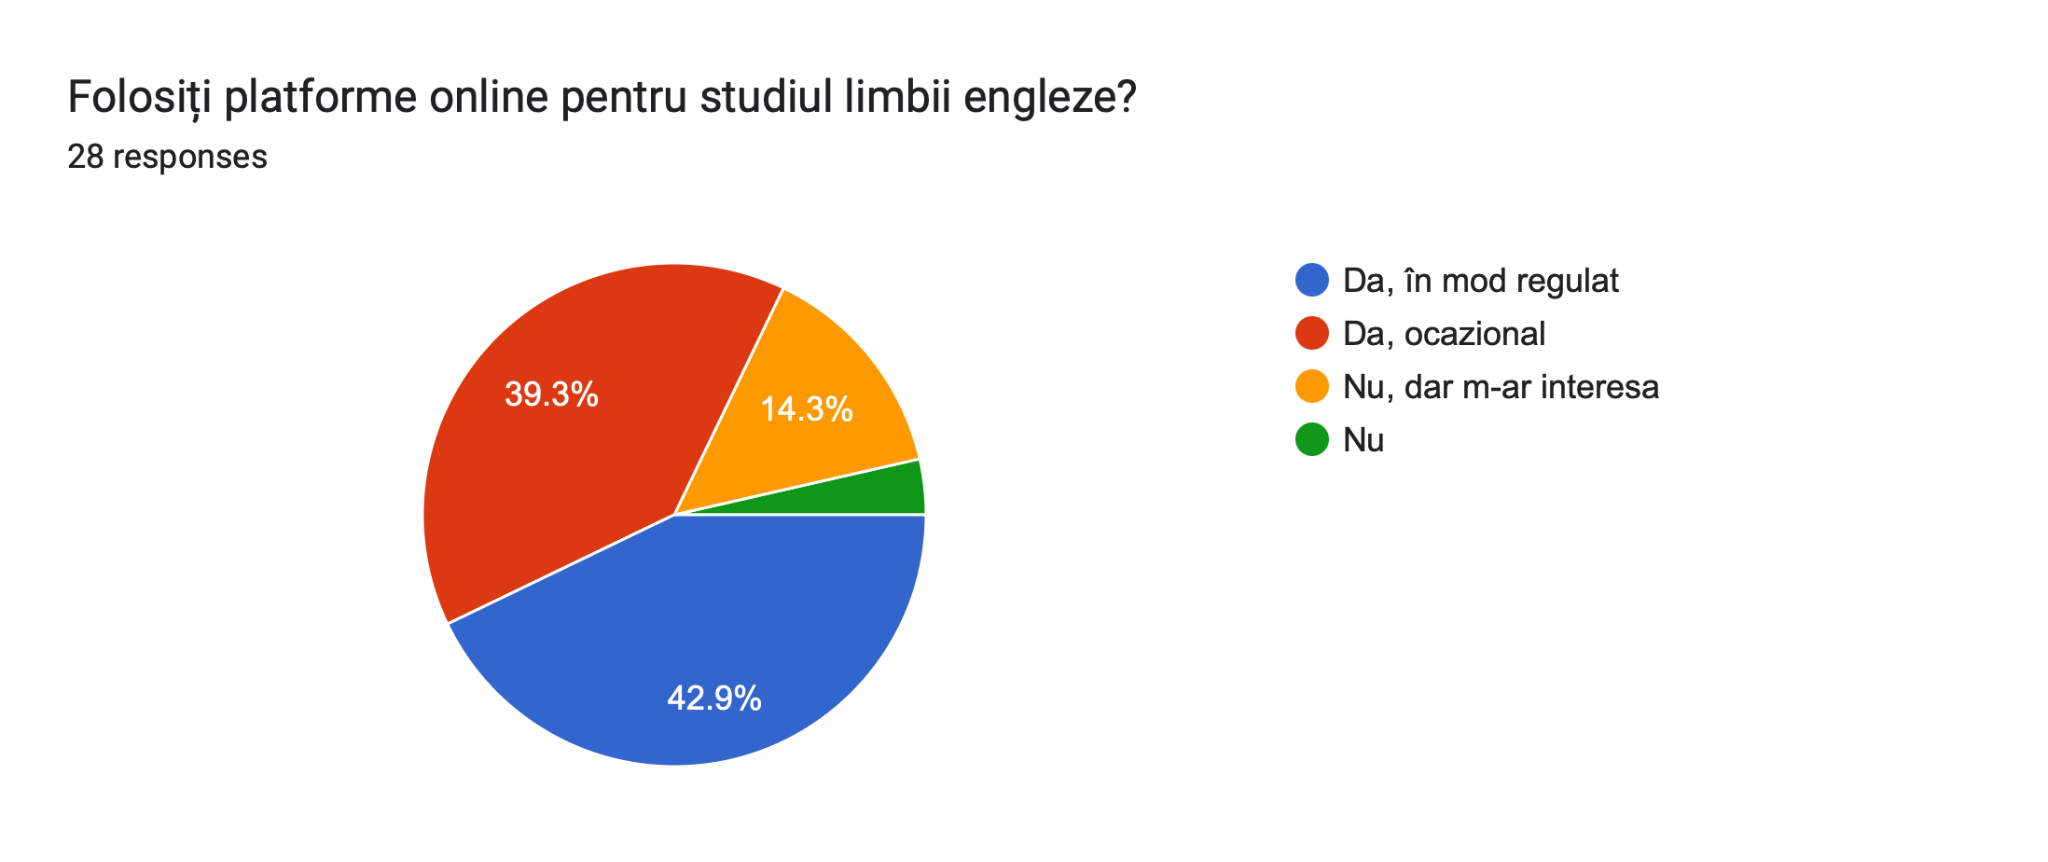
\includegraphics[width=\textwidth]{pics/survey/q01.png}
        \caption{Frecvența utilizării platformelor online pentru studiul limbii engleze}
        \label{fig:survey-q01}
    \end{subfigure}
    \hfill
    \begin{subfigure}{0.48\textwidth}
        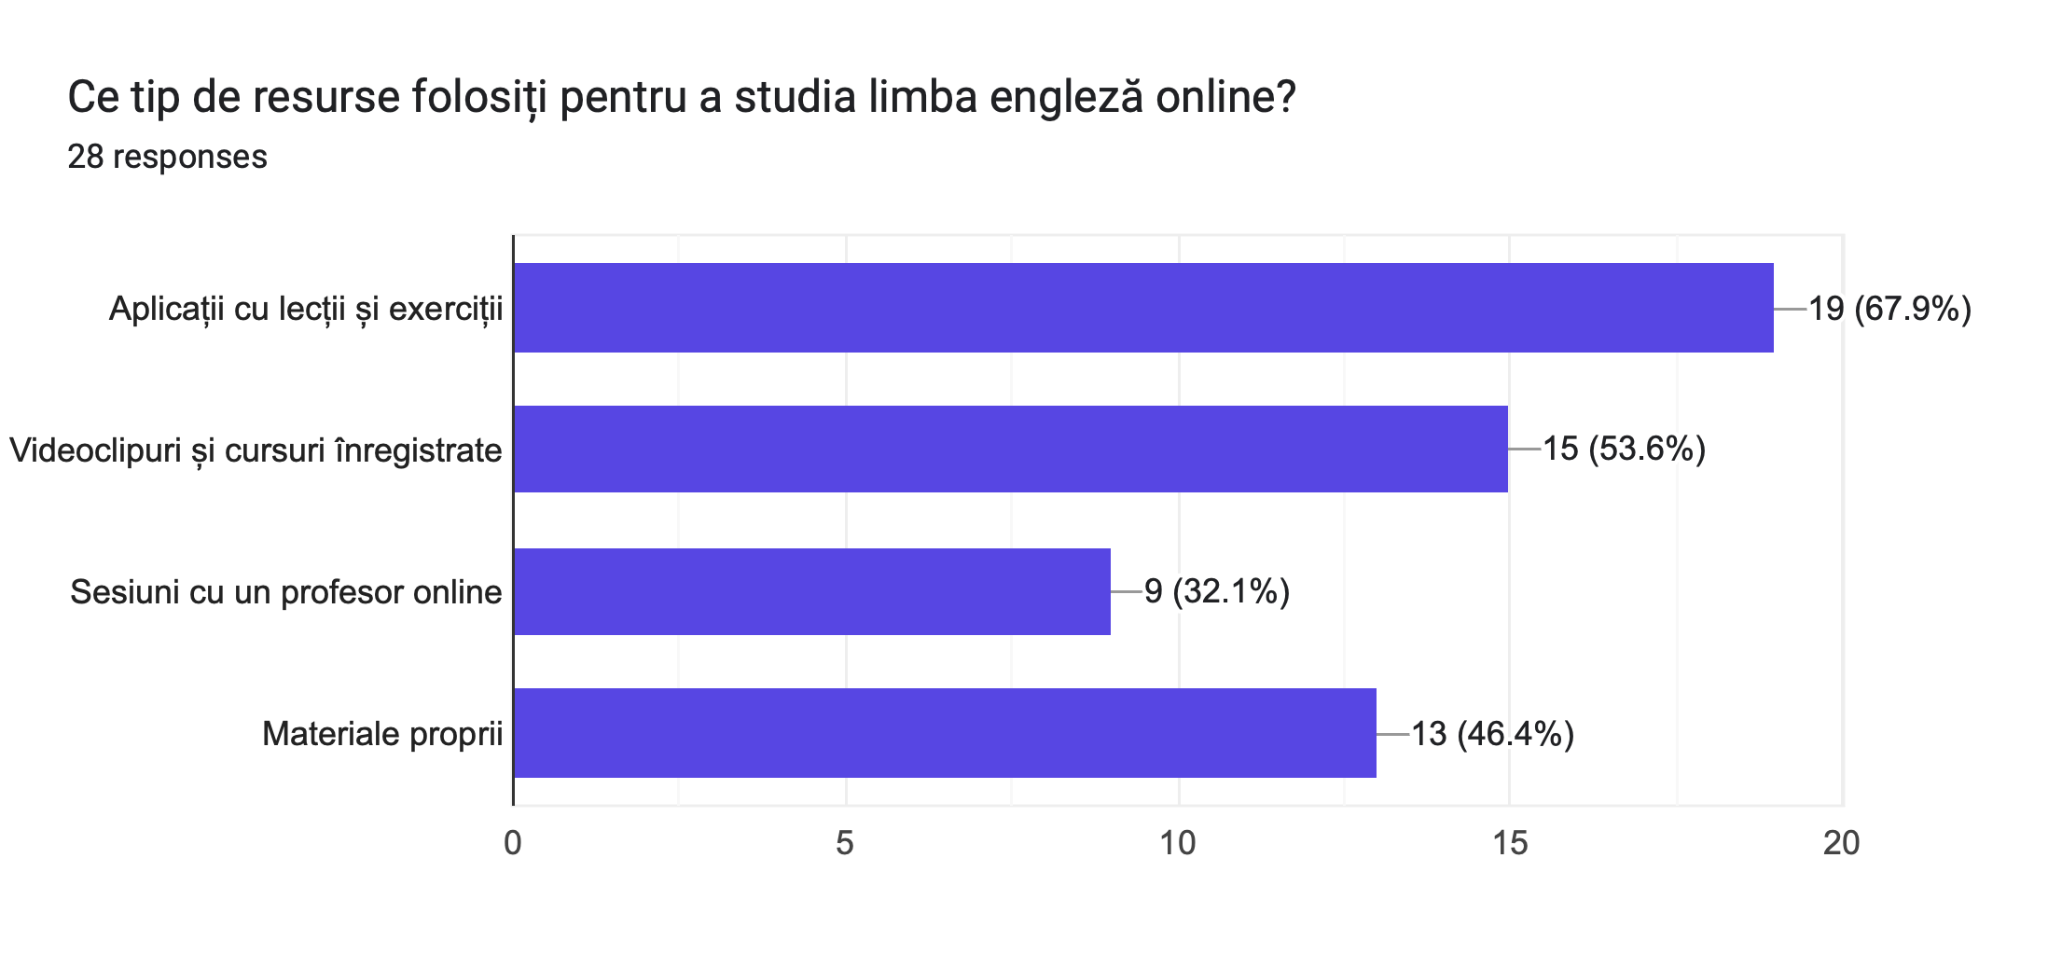
\includegraphics[width=\textwidth]{pics/survey/q02.png}
        \caption{Tipurile de resurse utilizate pentru studiul limbii engleze}
        \label{fig:survey-q02}
    \end{subfigure}
    \caption{Obiceiuri de studiu online}
\end{figure}

\begin{figure}[htbp]
    \centering
    \begin{subfigure}{0.48\textwidth}
        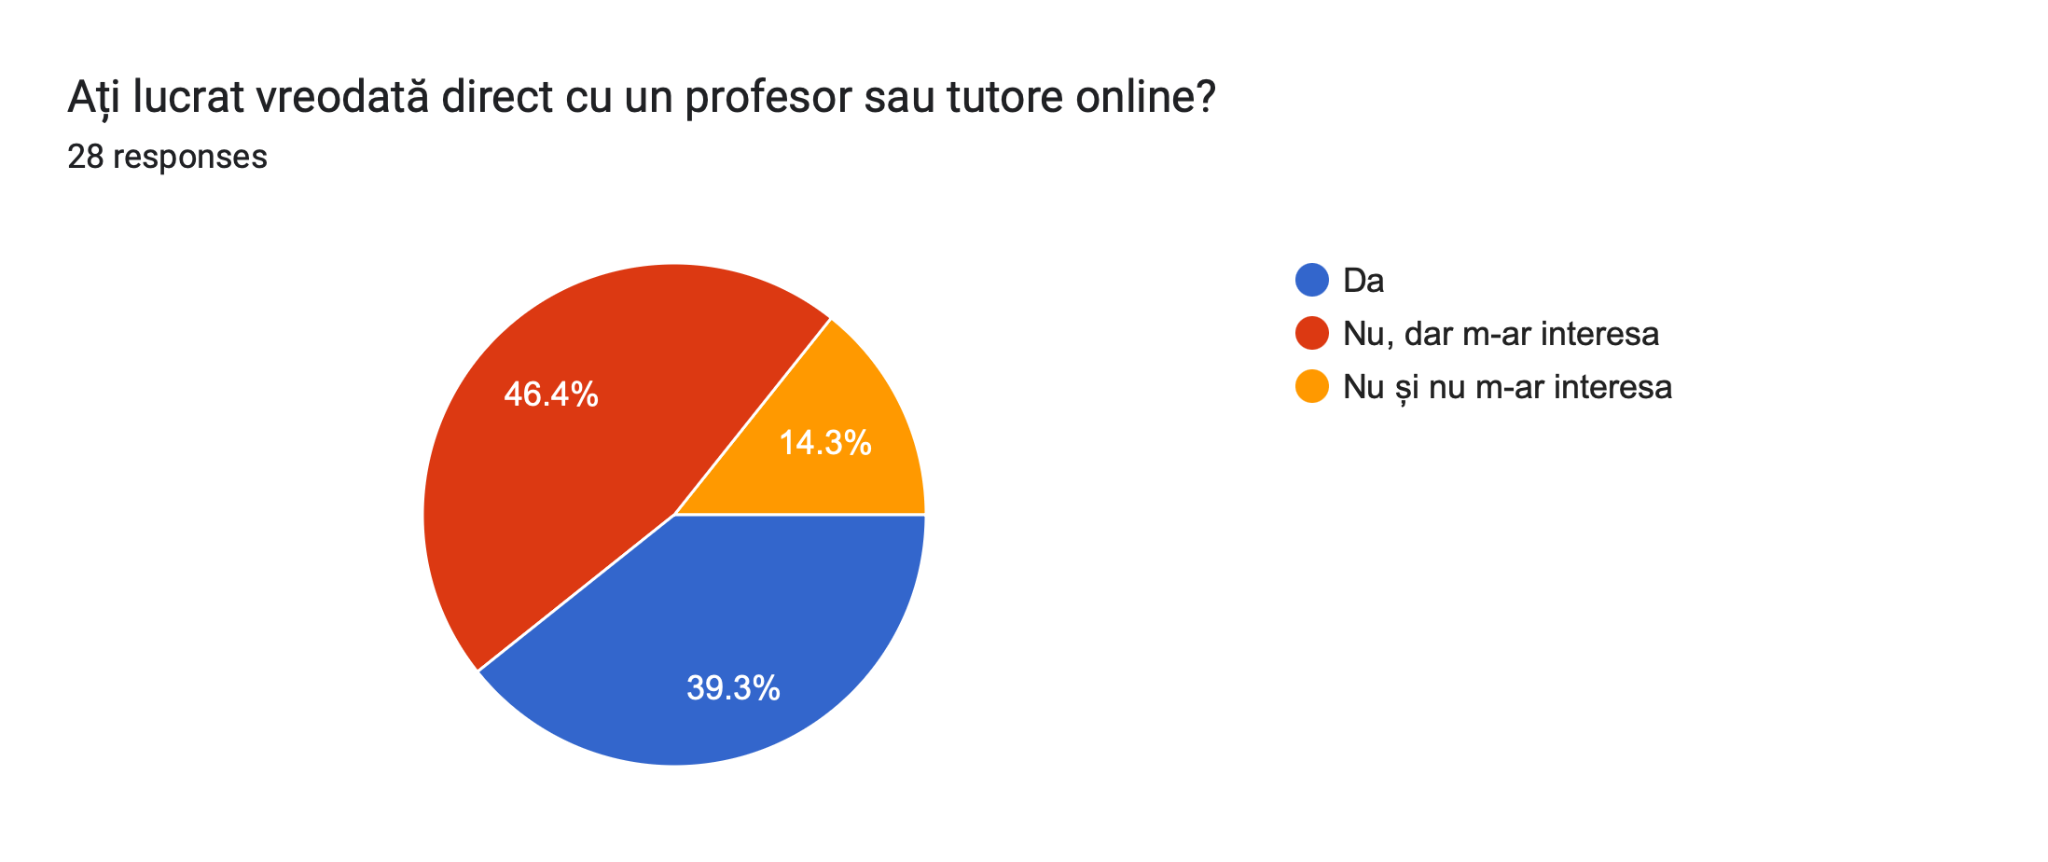
\includegraphics[width=\textwidth]{pics/survey/q03.png}
        \caption{Experiența anterioară cu meditațiile online}
        \label{fig:survey-q03}
    \end{subfigure}
    \hfill
    \begin{subfigure}{0.48\textwidth}
        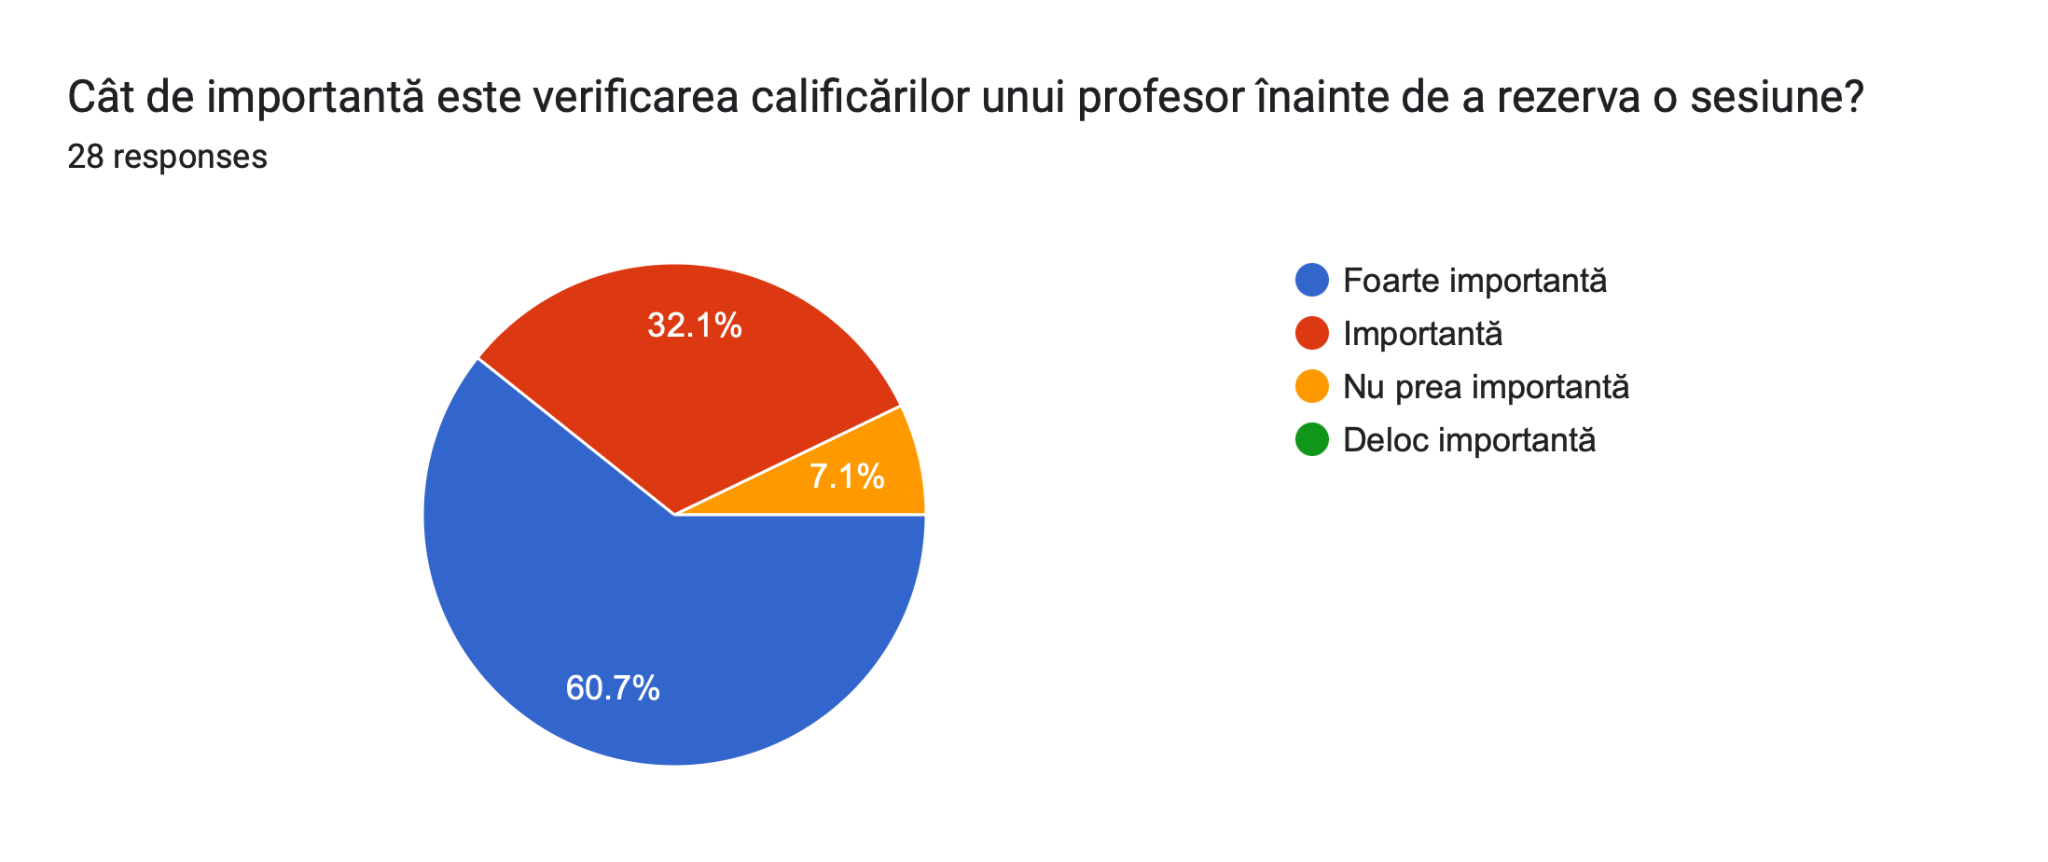
\includegraphics[width=\textwidth]{pics/survey/q06.png}
        \caption{Importanța verificării calificărilor unui profesor înainte de rezervare}
        \label{fig:survey-q06}
    \end{subfigure}
    \caption{Percepția asupra sesiunilor cu profesori}
\end{figure}

\begin{figure}[htbp]
    \centering
    \begin{subfigure}{0.48\textwidth}
        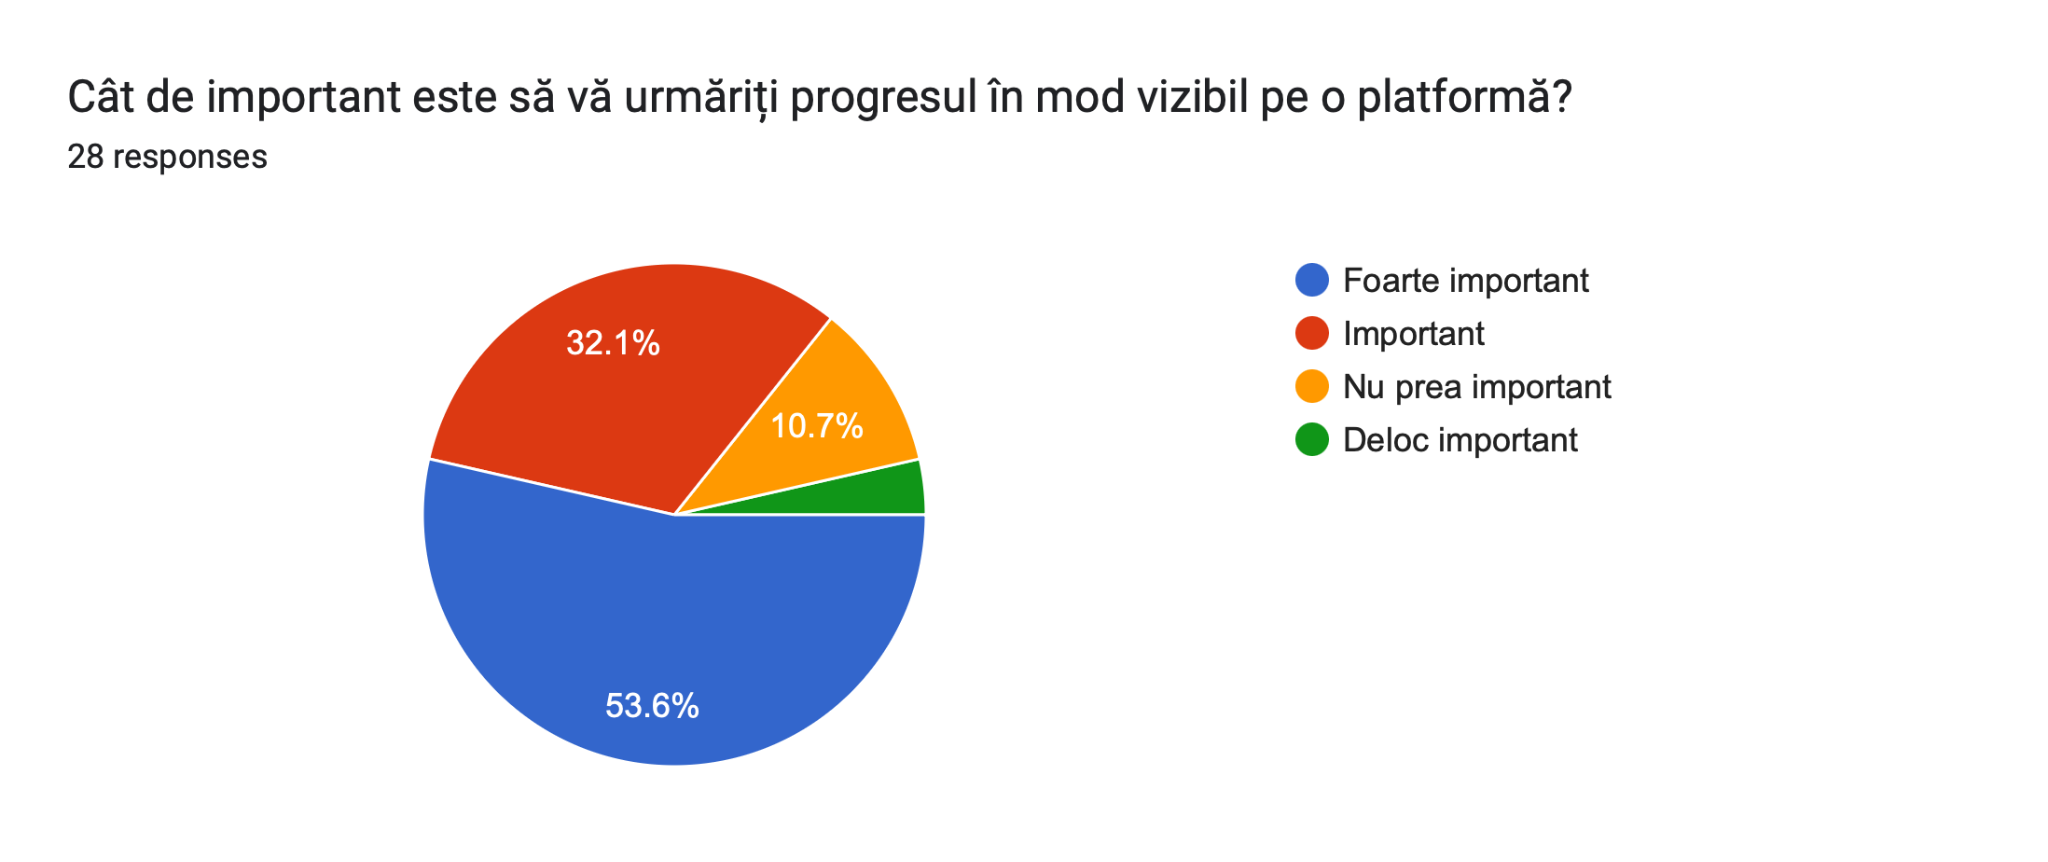
\includegraphics[width=\textwidth]{pics/survey/q05.png}
        \caption{Importanța urmăririi progresului pe o platformă educațională}
        \label{fig:survey-q05}
    \end{subfigure}
    \hfill
    \begin{subfigure}{0.48\textwidth}
        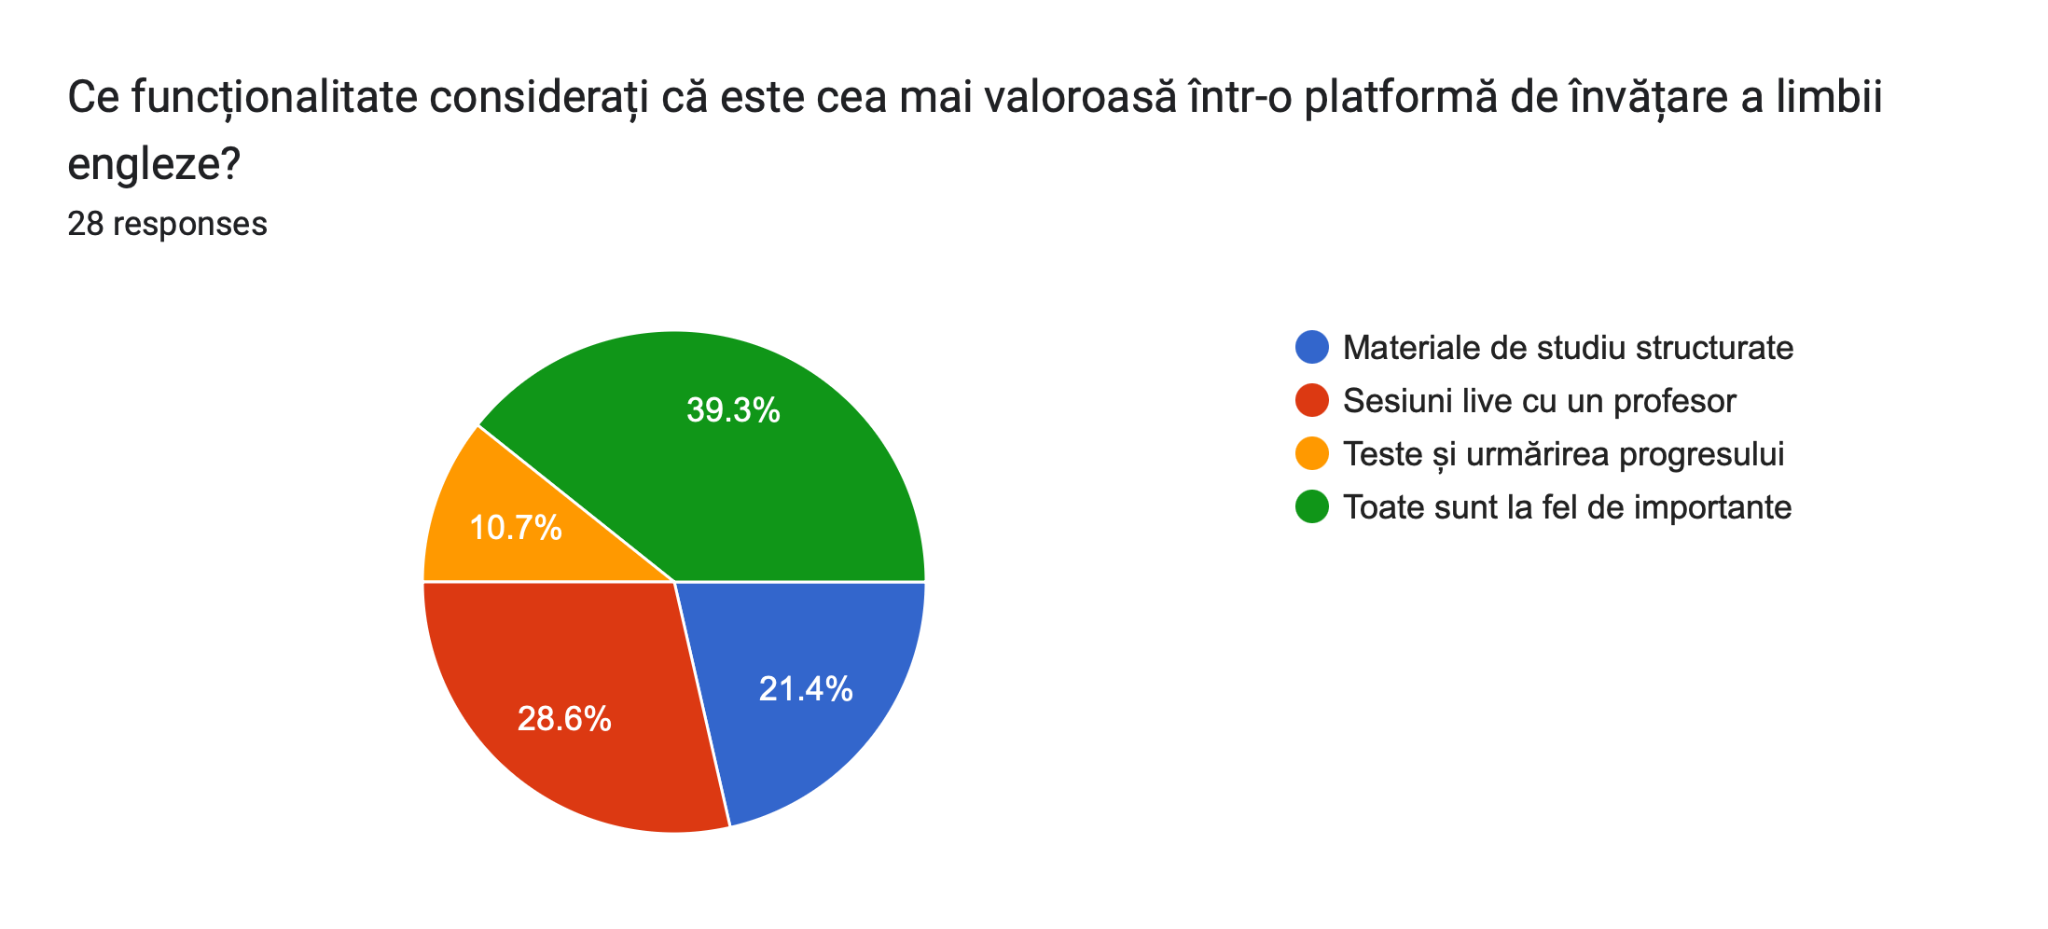
\includegraphics[width=\textwidth]{pics/survey/q08.png}
        \caption{Funcționalitatea considerată cea mai valoroasă pe o platformă de învățare}
        \label{fig:survey-q08}
    \end{subfigure}
    \caption{Preferințe față de funcționalitățile platformei}
\end{figure}

    \chapter{Diagrama entitate-relație a bazei de date}

\begin{figure}[htbp]
    \centering
    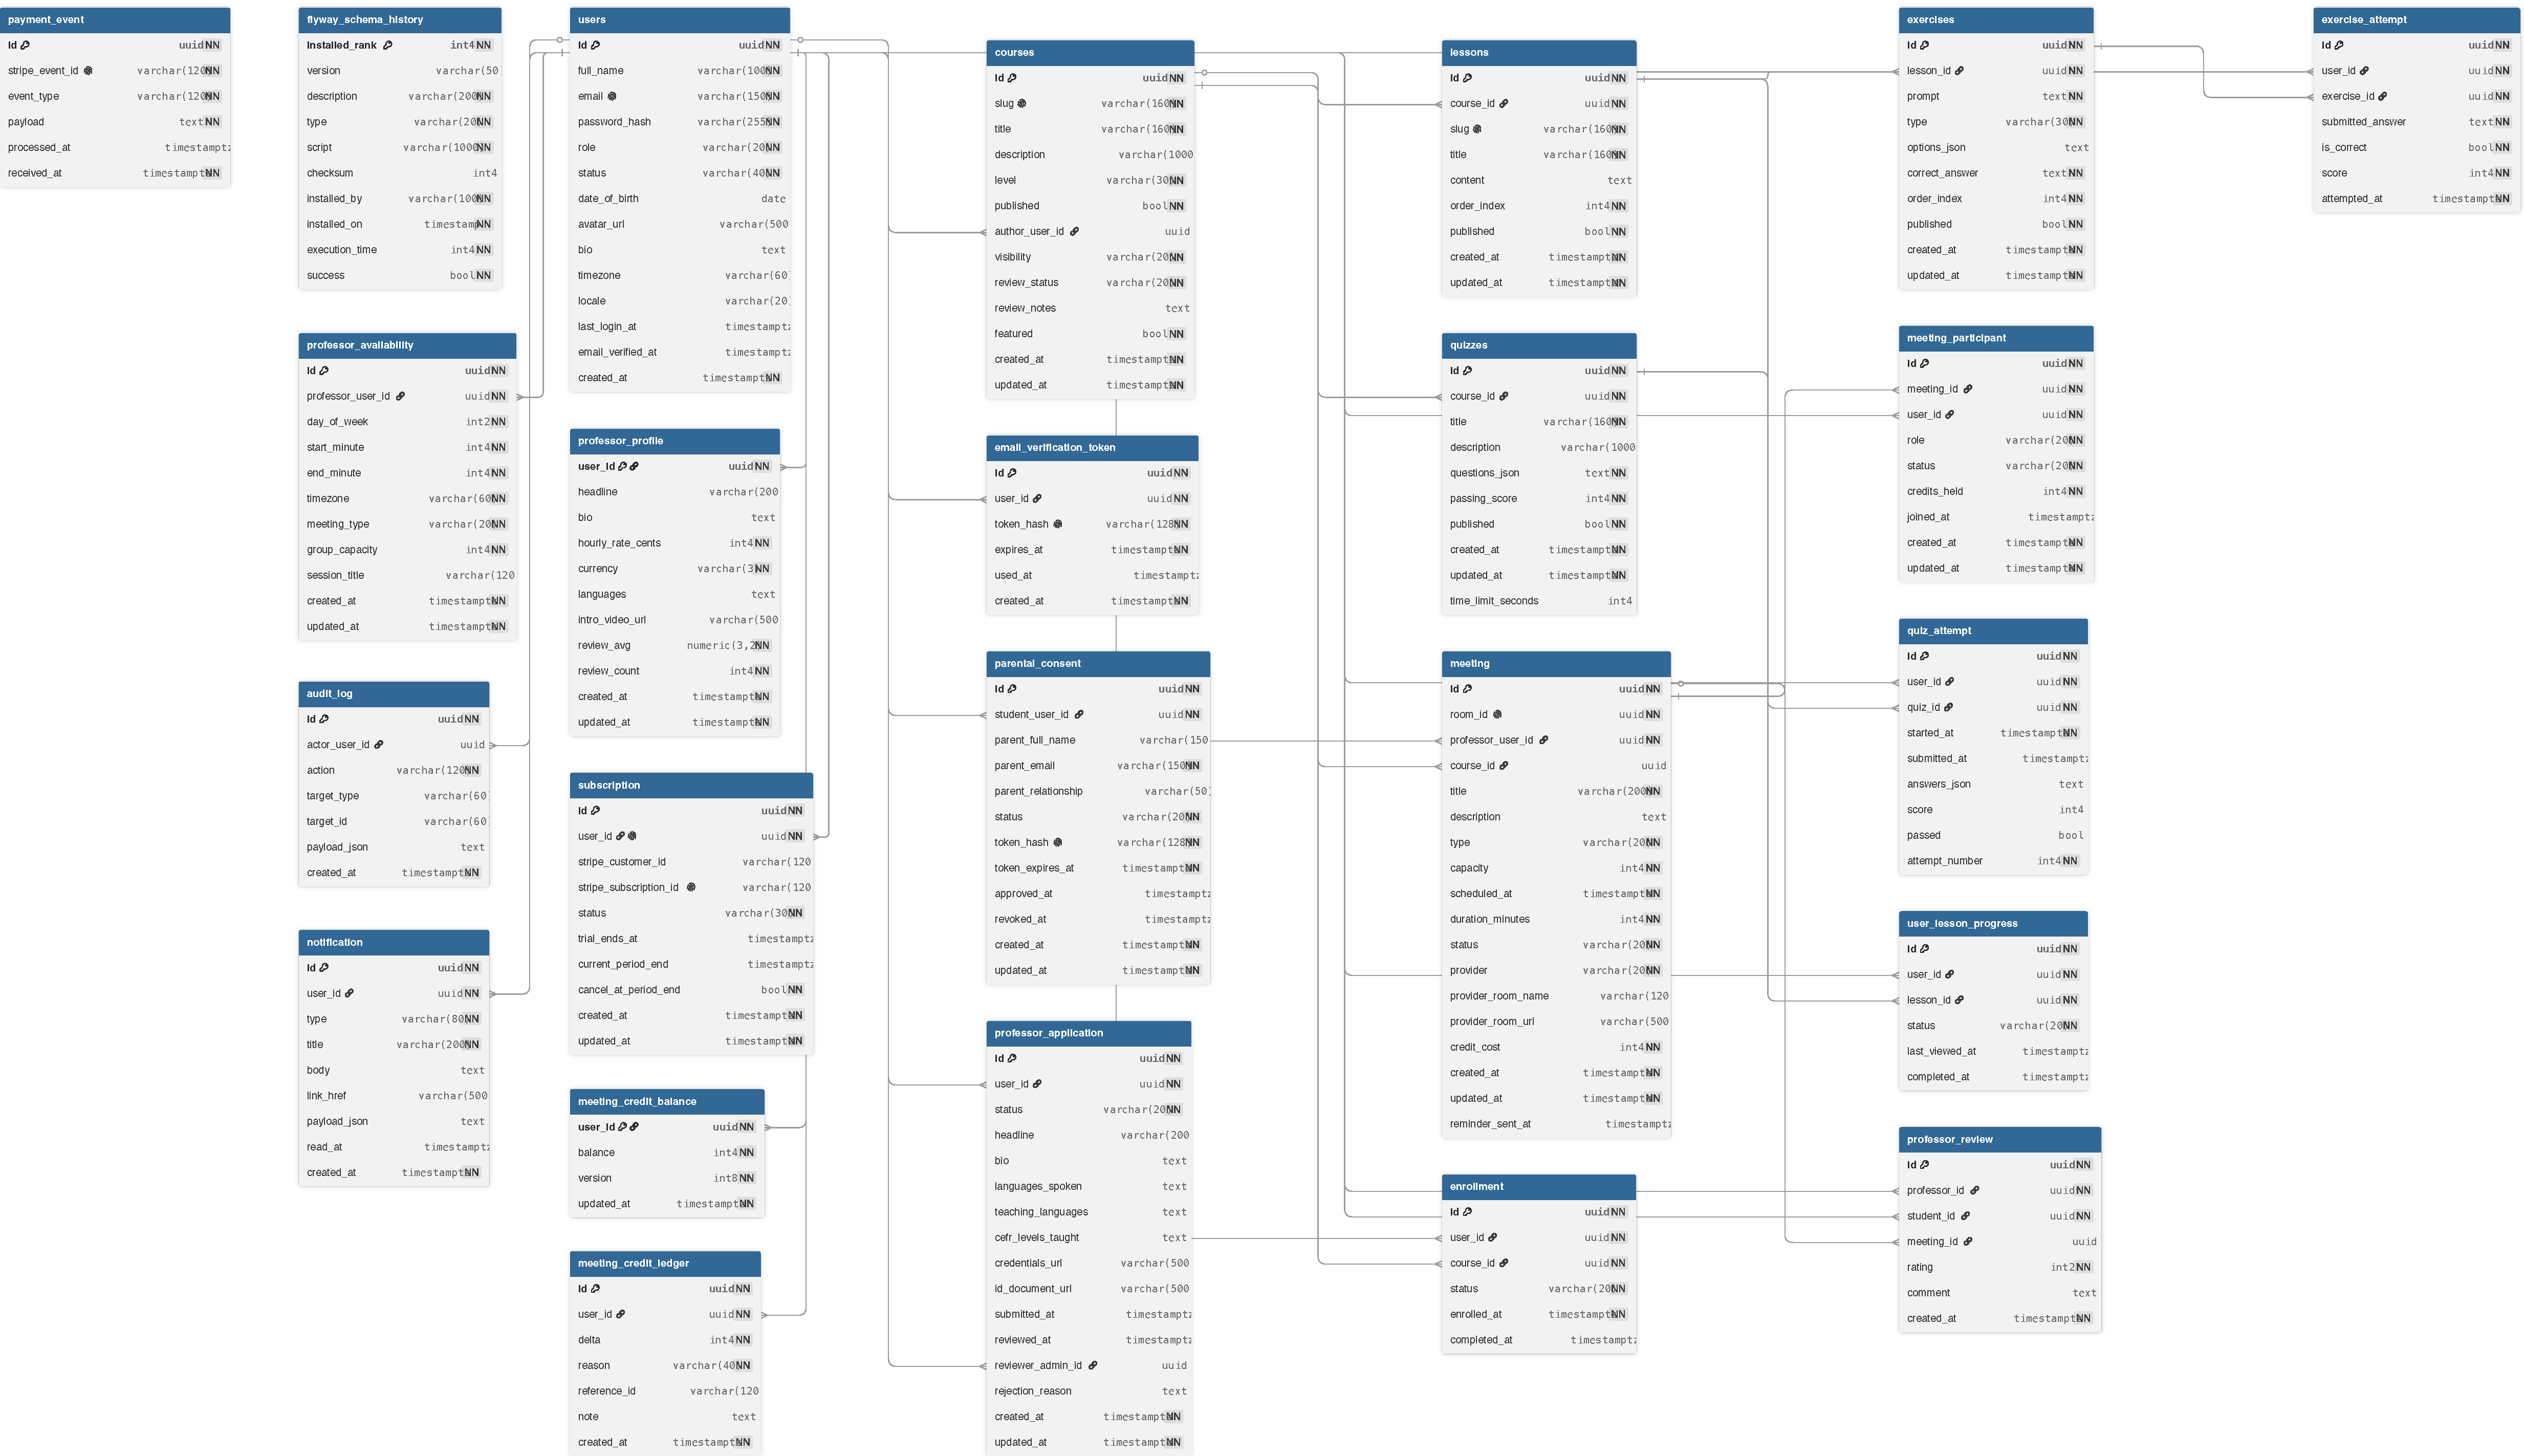
\includegraphics[width=0.8\textwidth]{pics/diagrams/er-diagram.pdf}
    \caption{Diagrama entitate-relație a bazei de date}
    \label{fig:er-diagram}
\end{figure}

    \chapter{Capturi de ecran ale aplicației}

\begin{figure}[htbp]
    \centering
    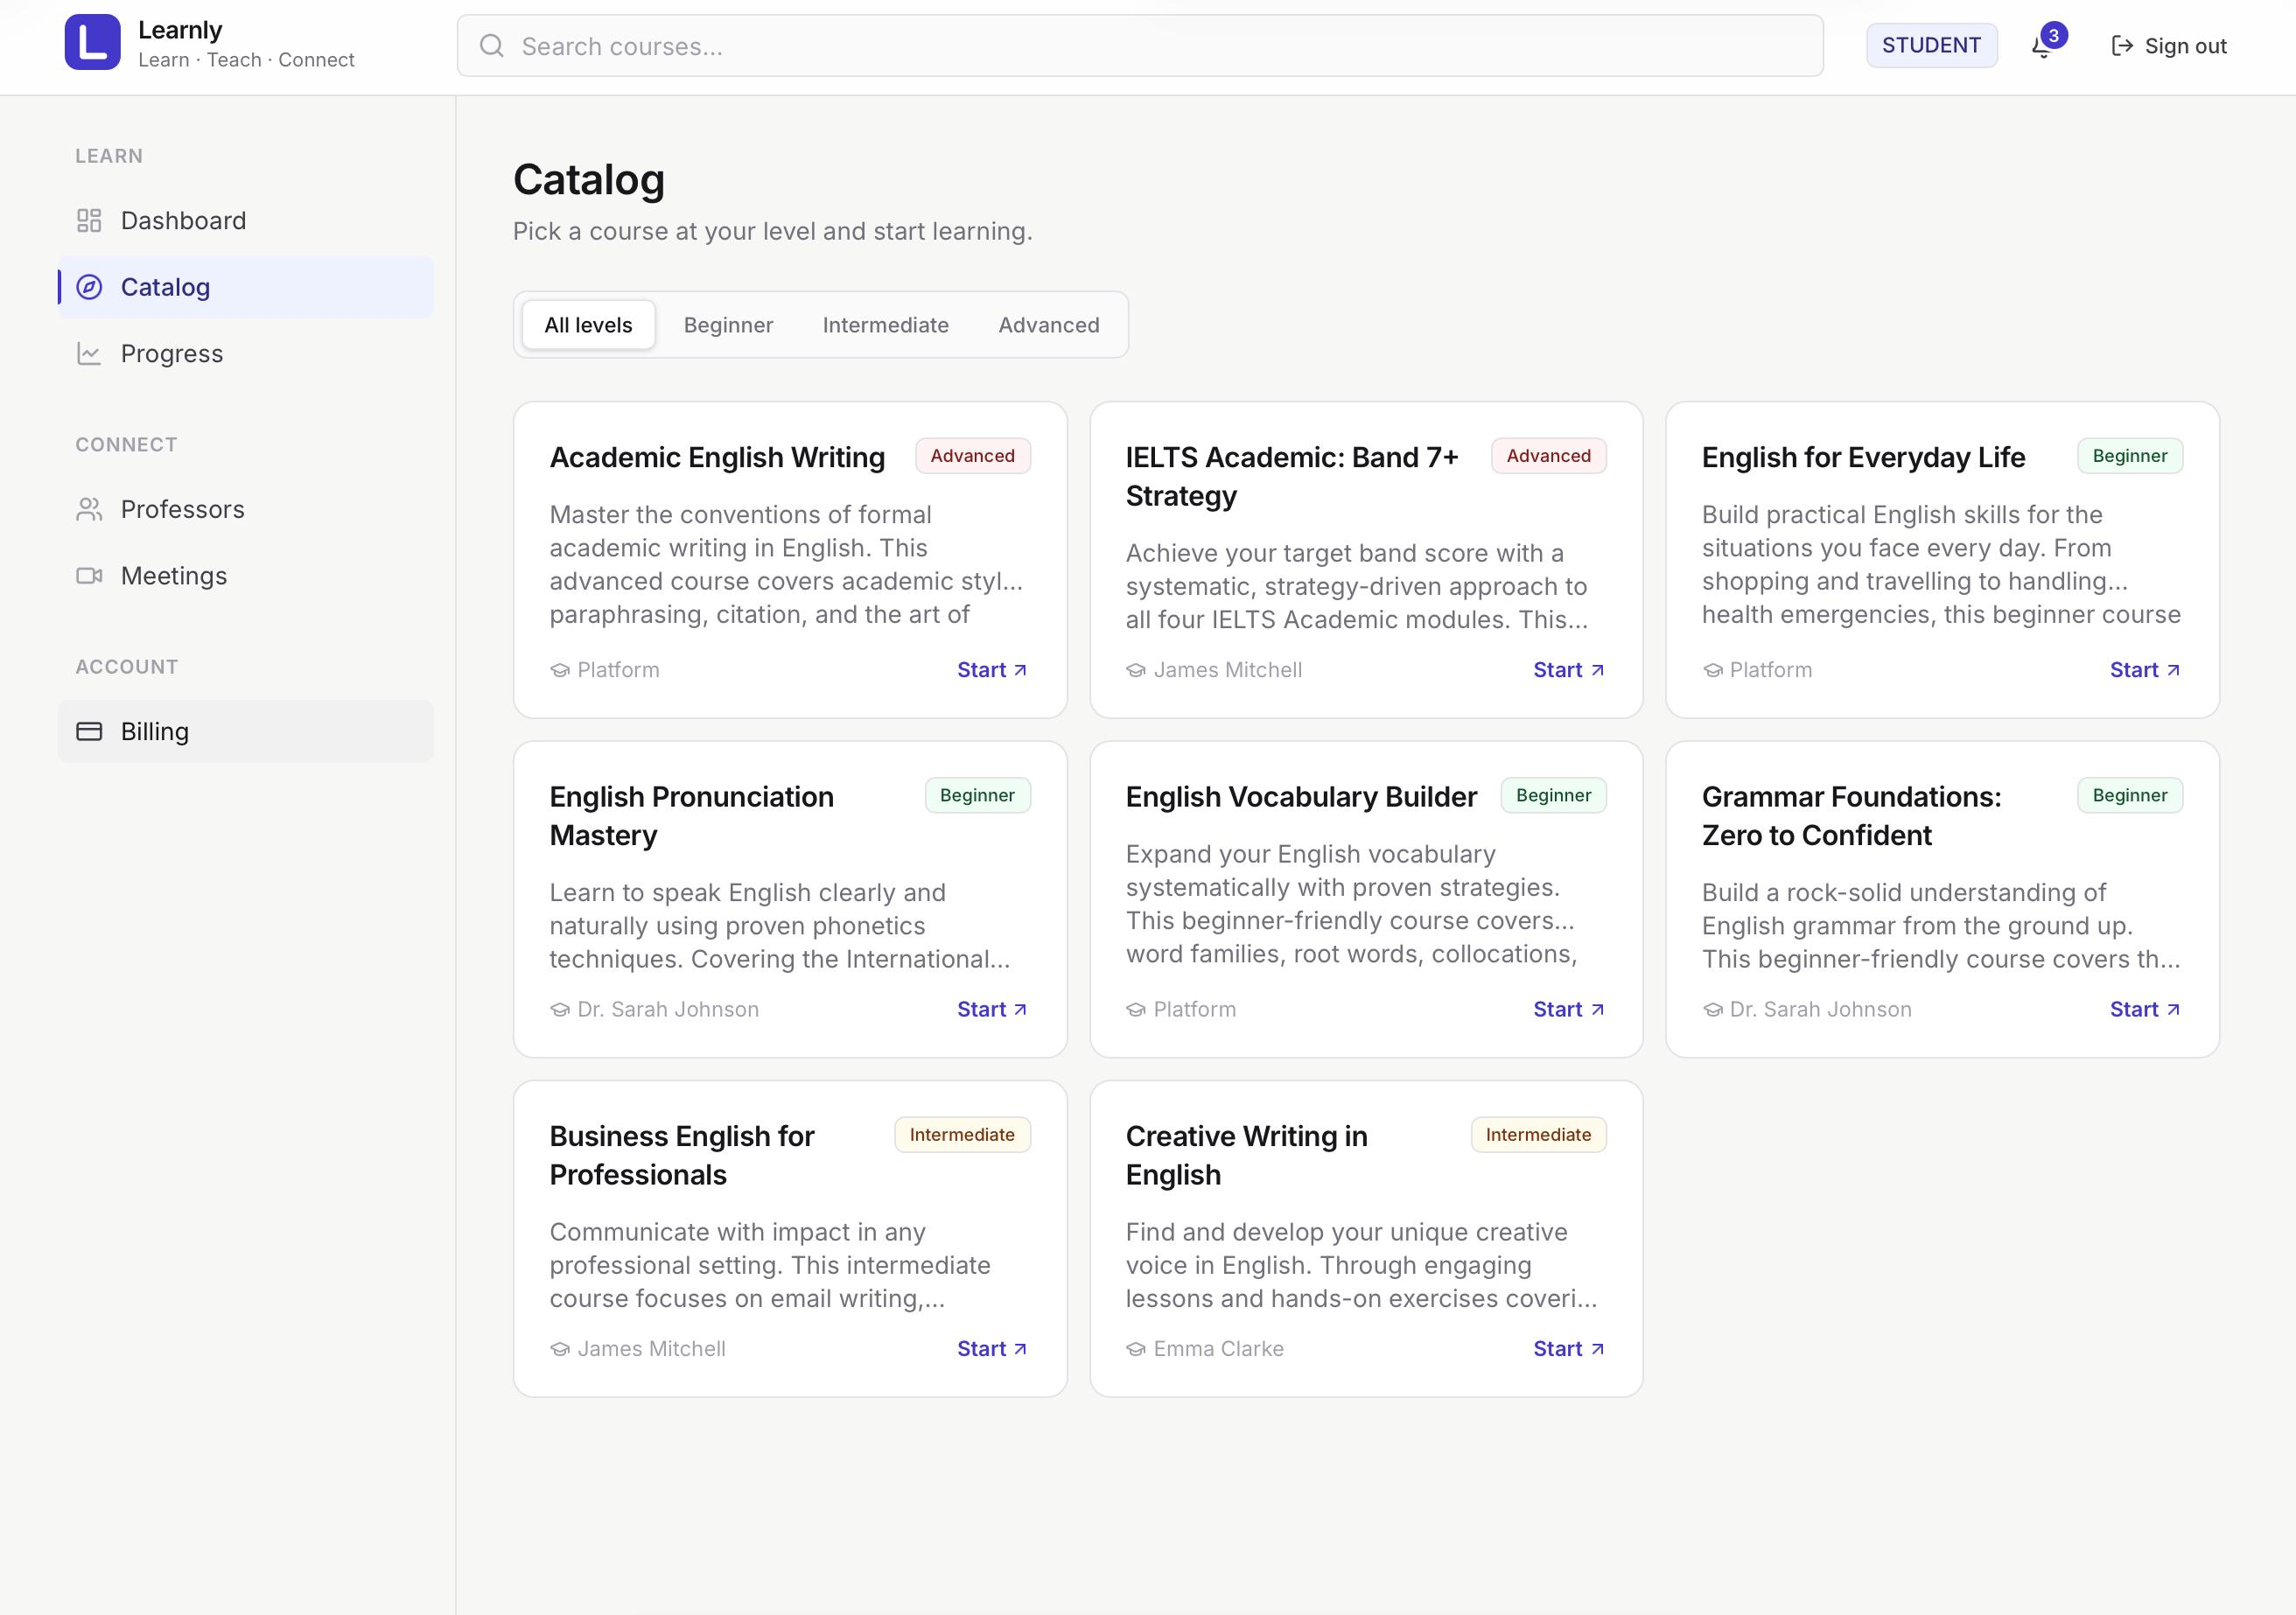
\includegraphics[width=\textwidth]{pics/screenshots/catalog.jpeg}
    \caption{Catalogul de cursuri}
    \label{fig:catalog}
\end{figure}

\begin{figure}[htbp]
    \centering
    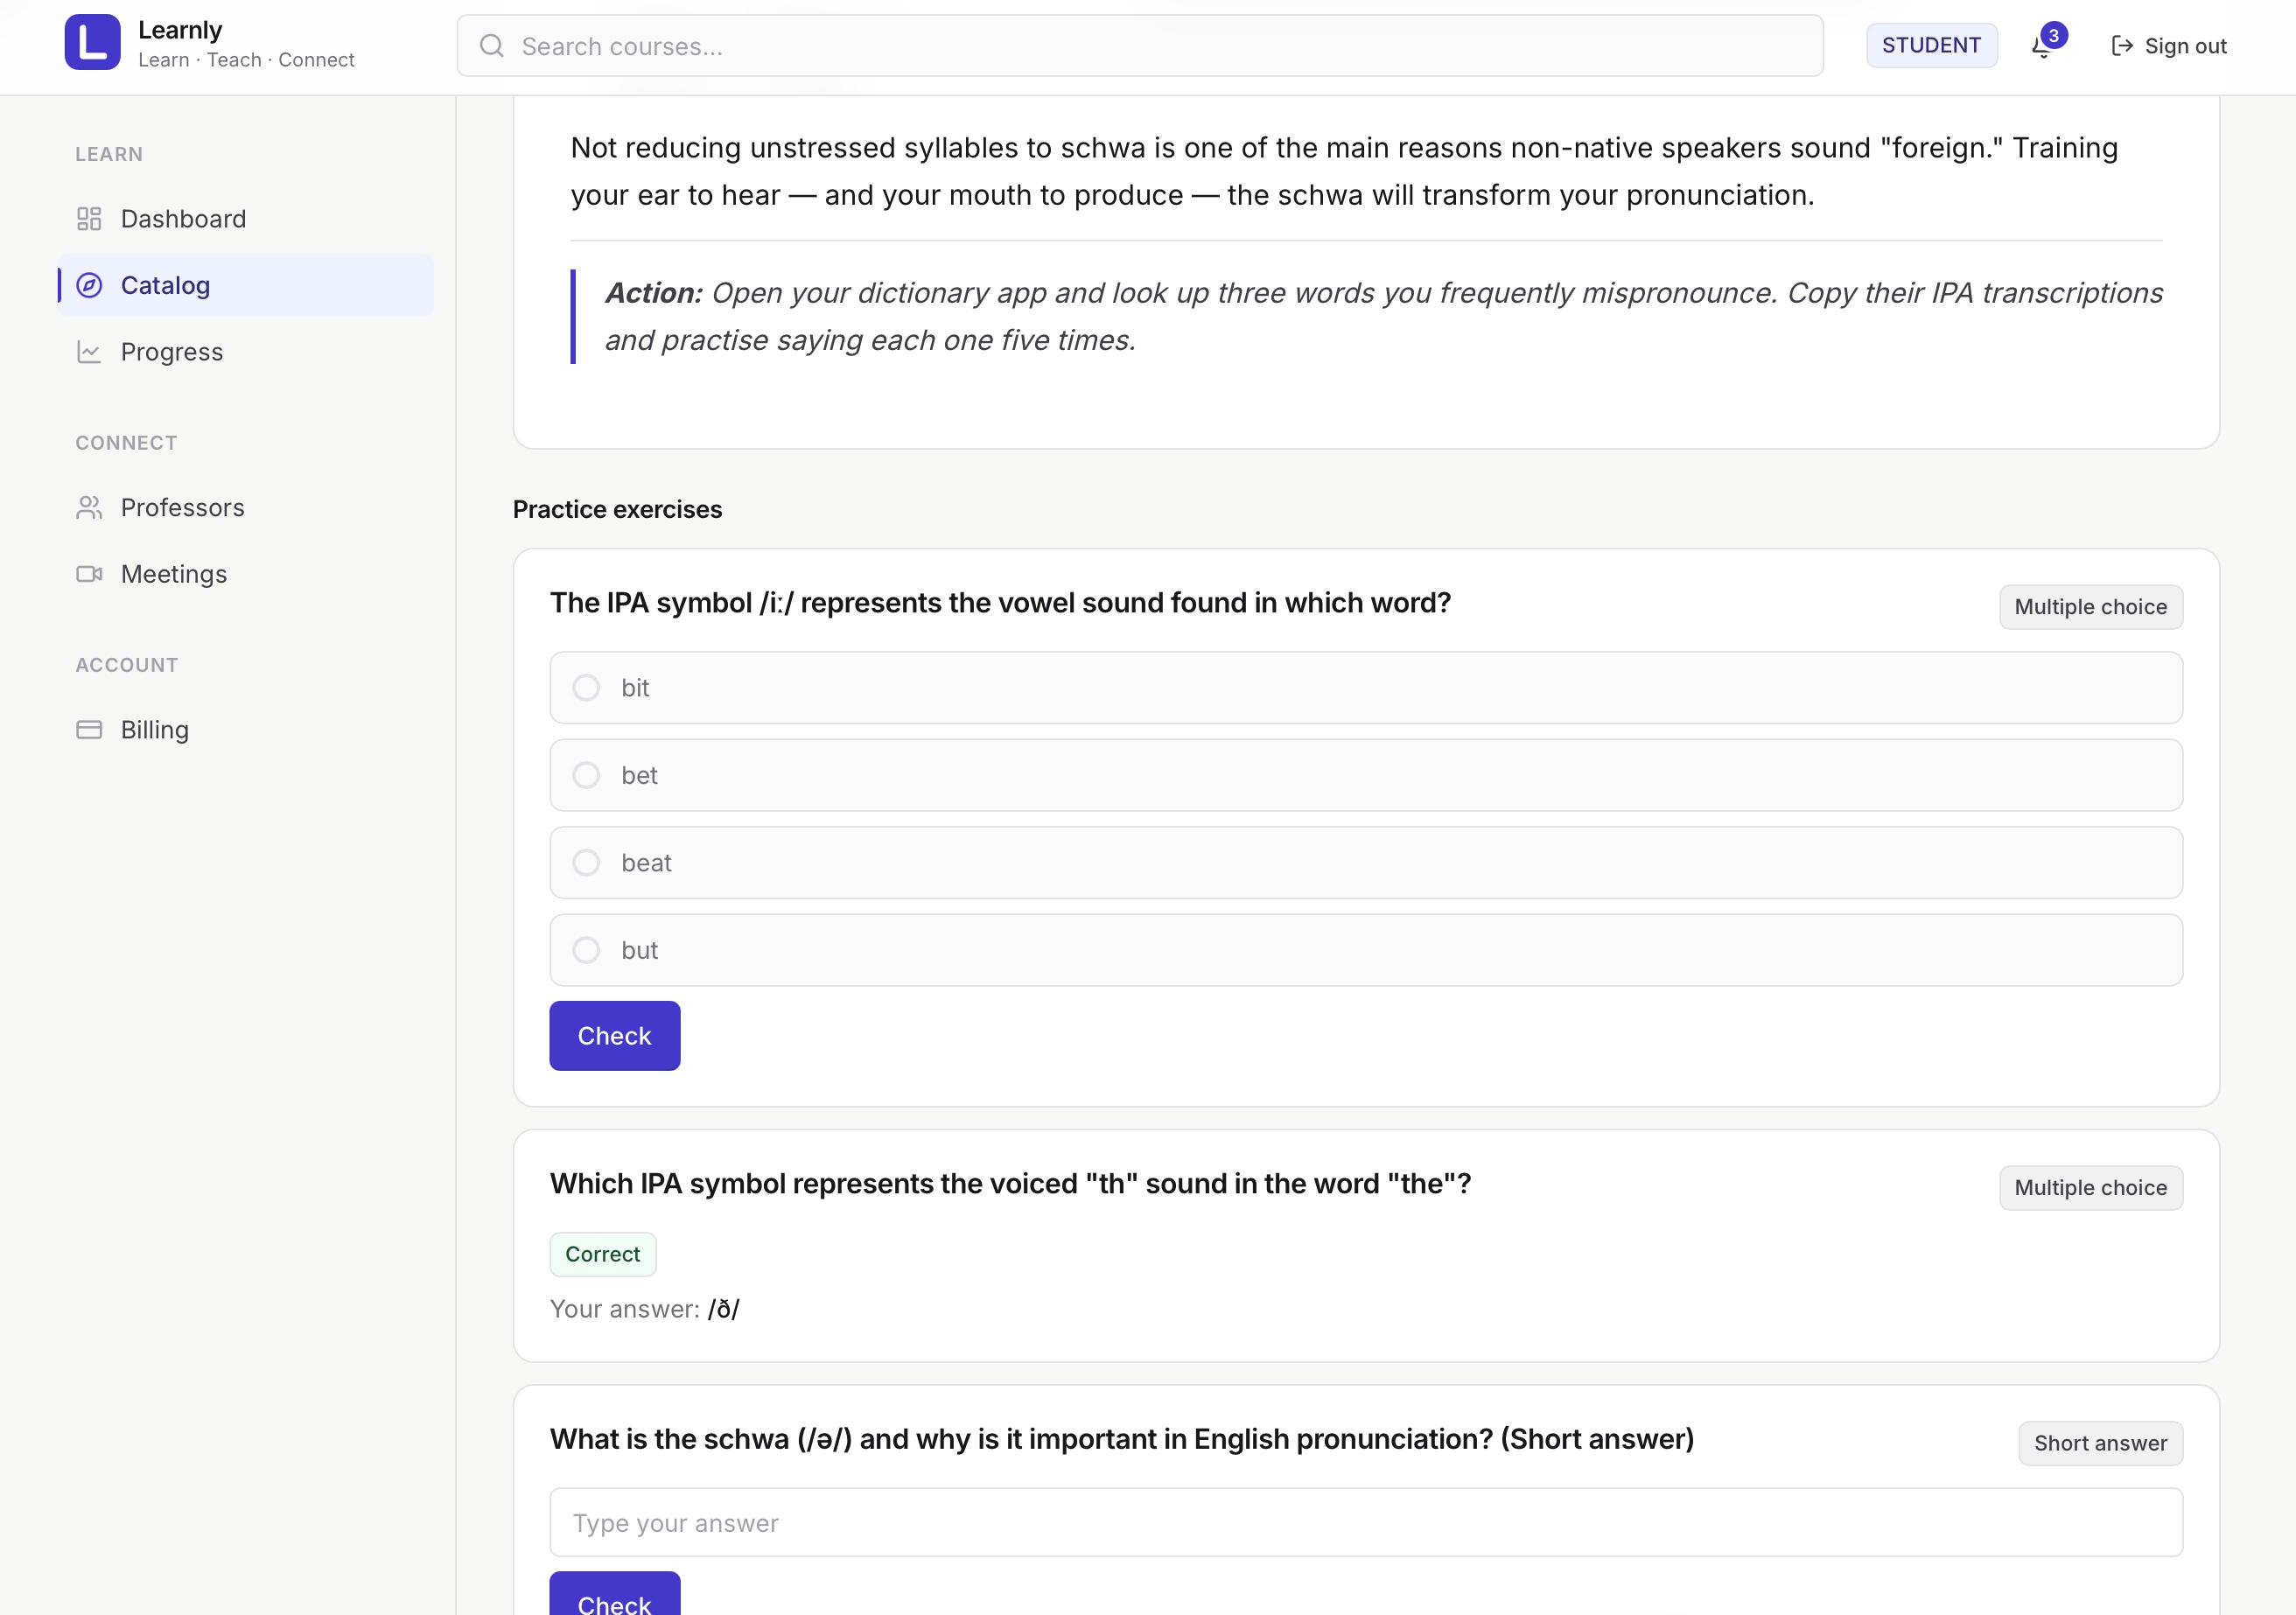
\includegraphics[width=\textwidth]{pics/screenshots/lesson-exercises.jpeg}
    \caption{O lecție cu exerciții interactive}
    \label{fig:lesson-exercises}
\end{figure}

\begin{figure}[htbp]
    \centering
    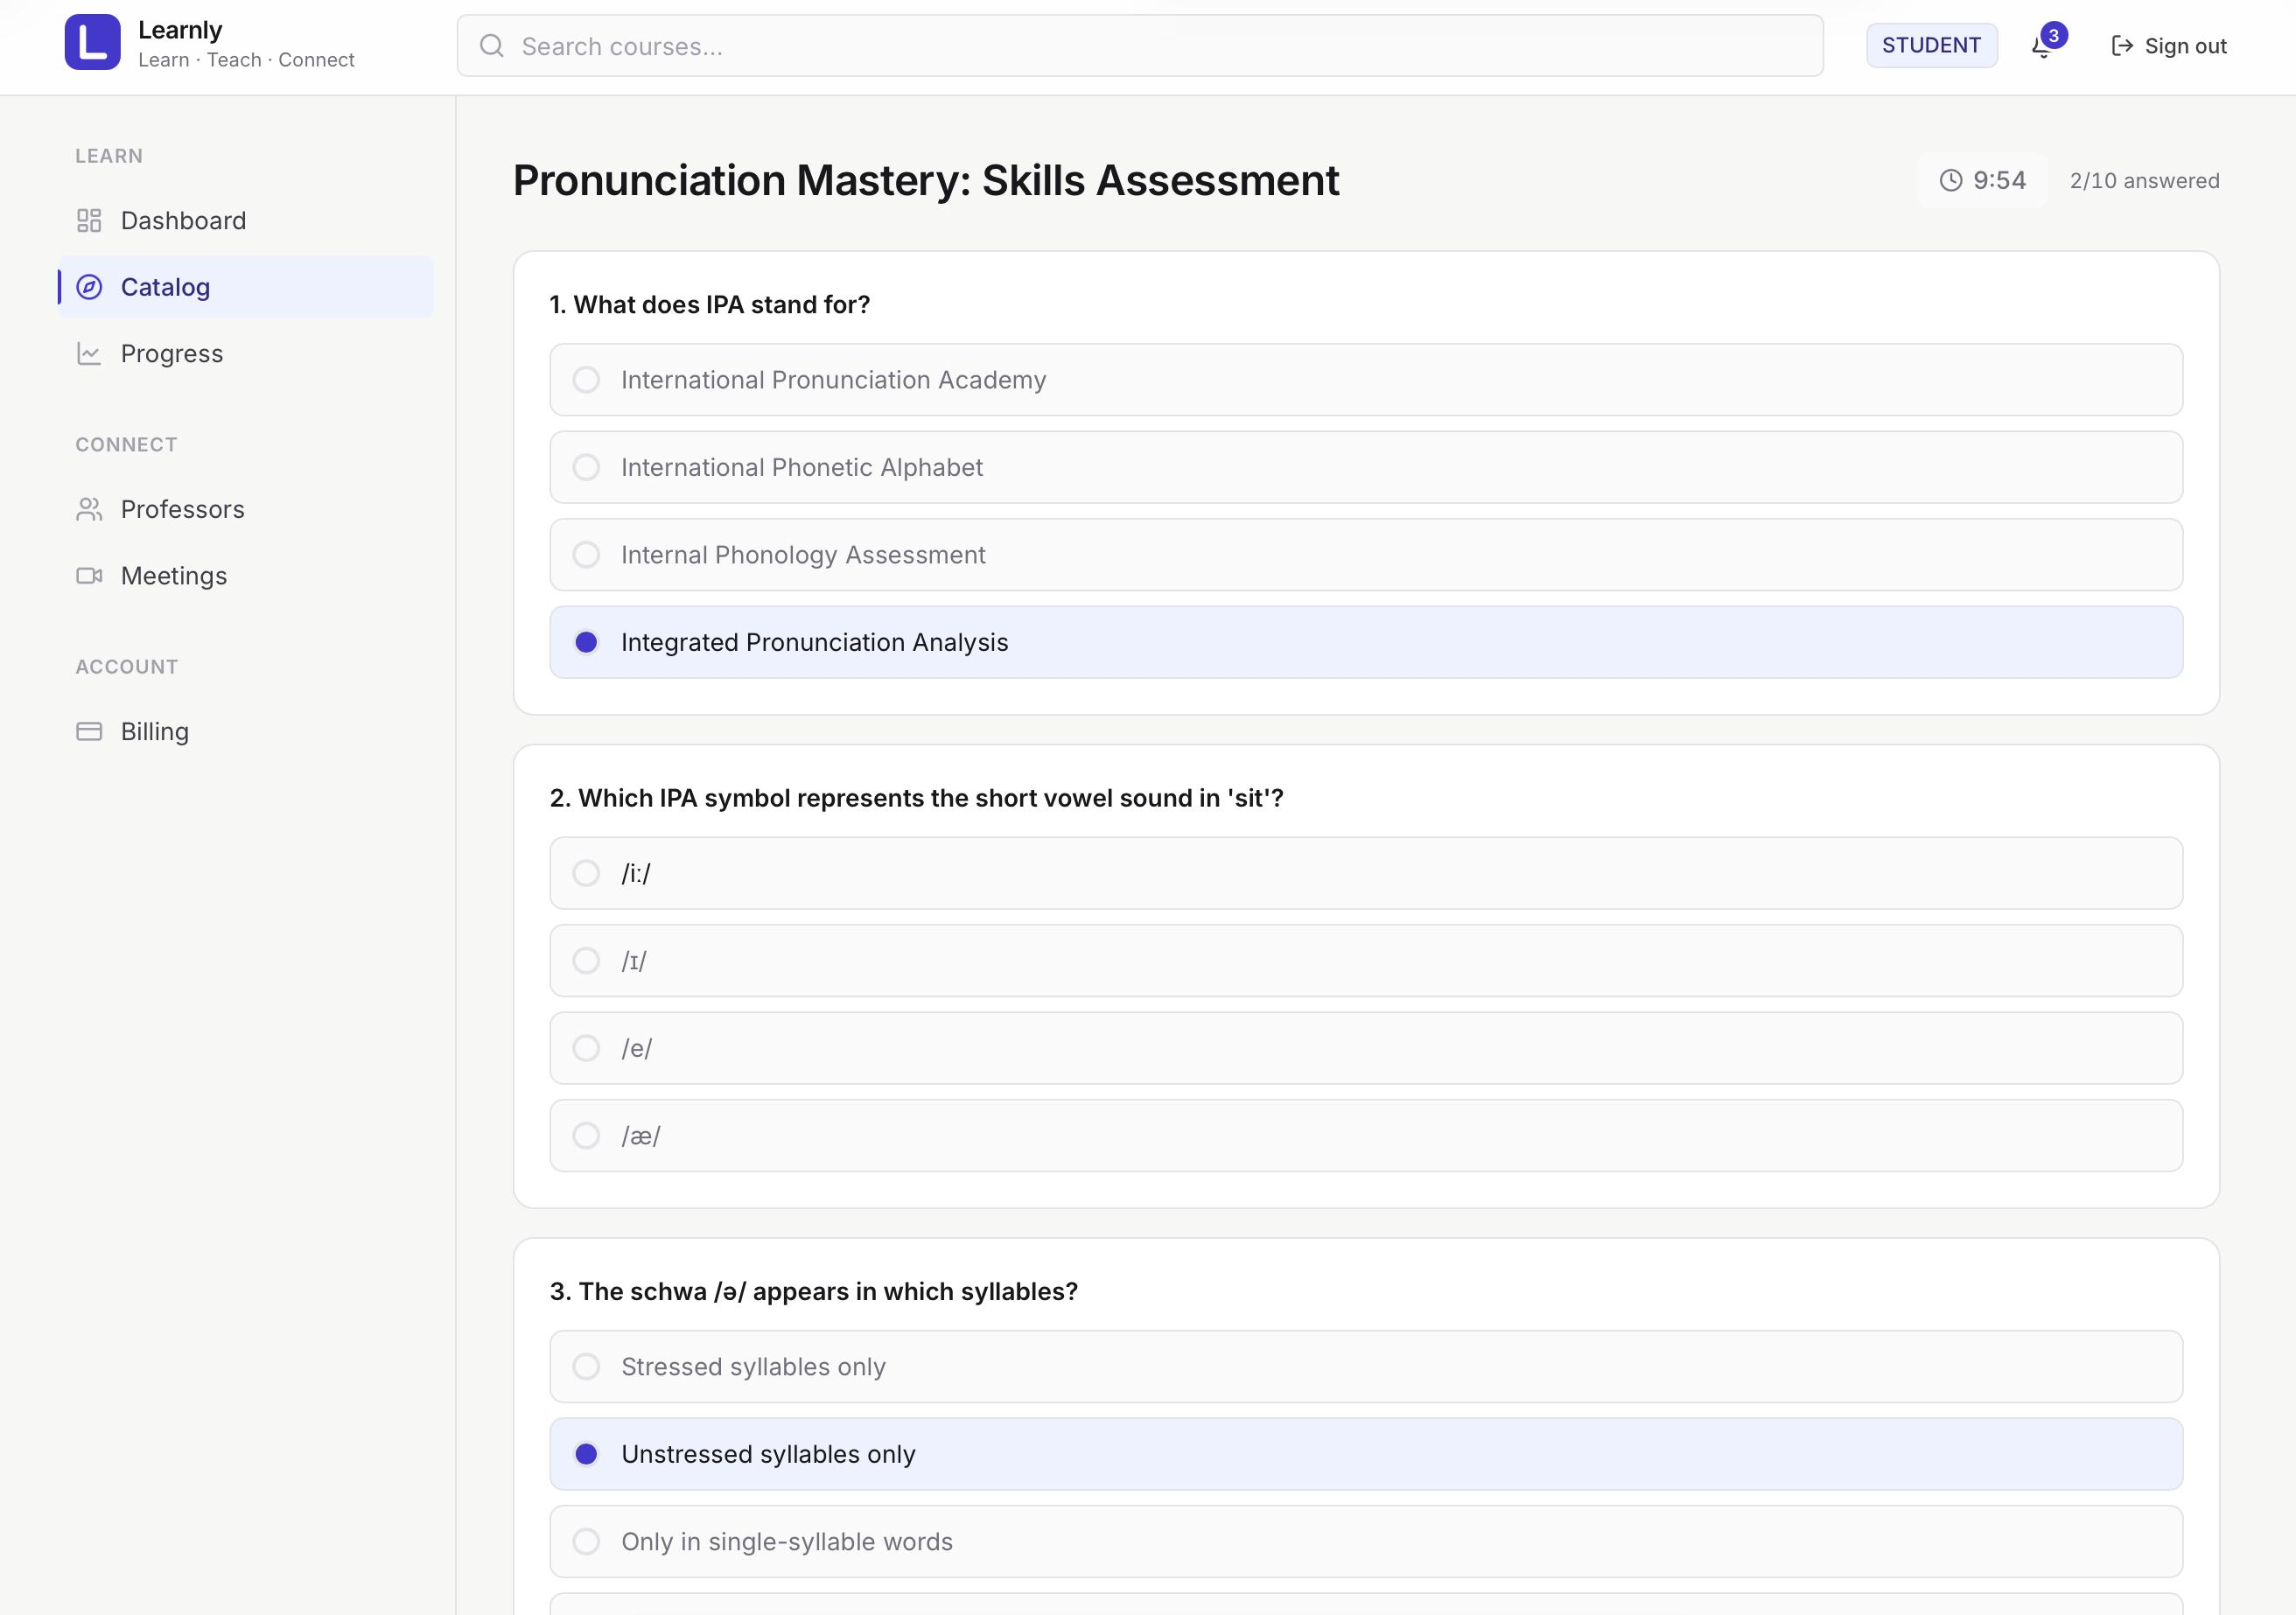
\includegraphics[width=\textwidth]{pics/screenshots/quiz.jpeg}
    \caption{Susținerea unui test cronometrat}
    \label{fig:quiz}
\end{figure}

\begin{figure}[htbp]
    \centering
    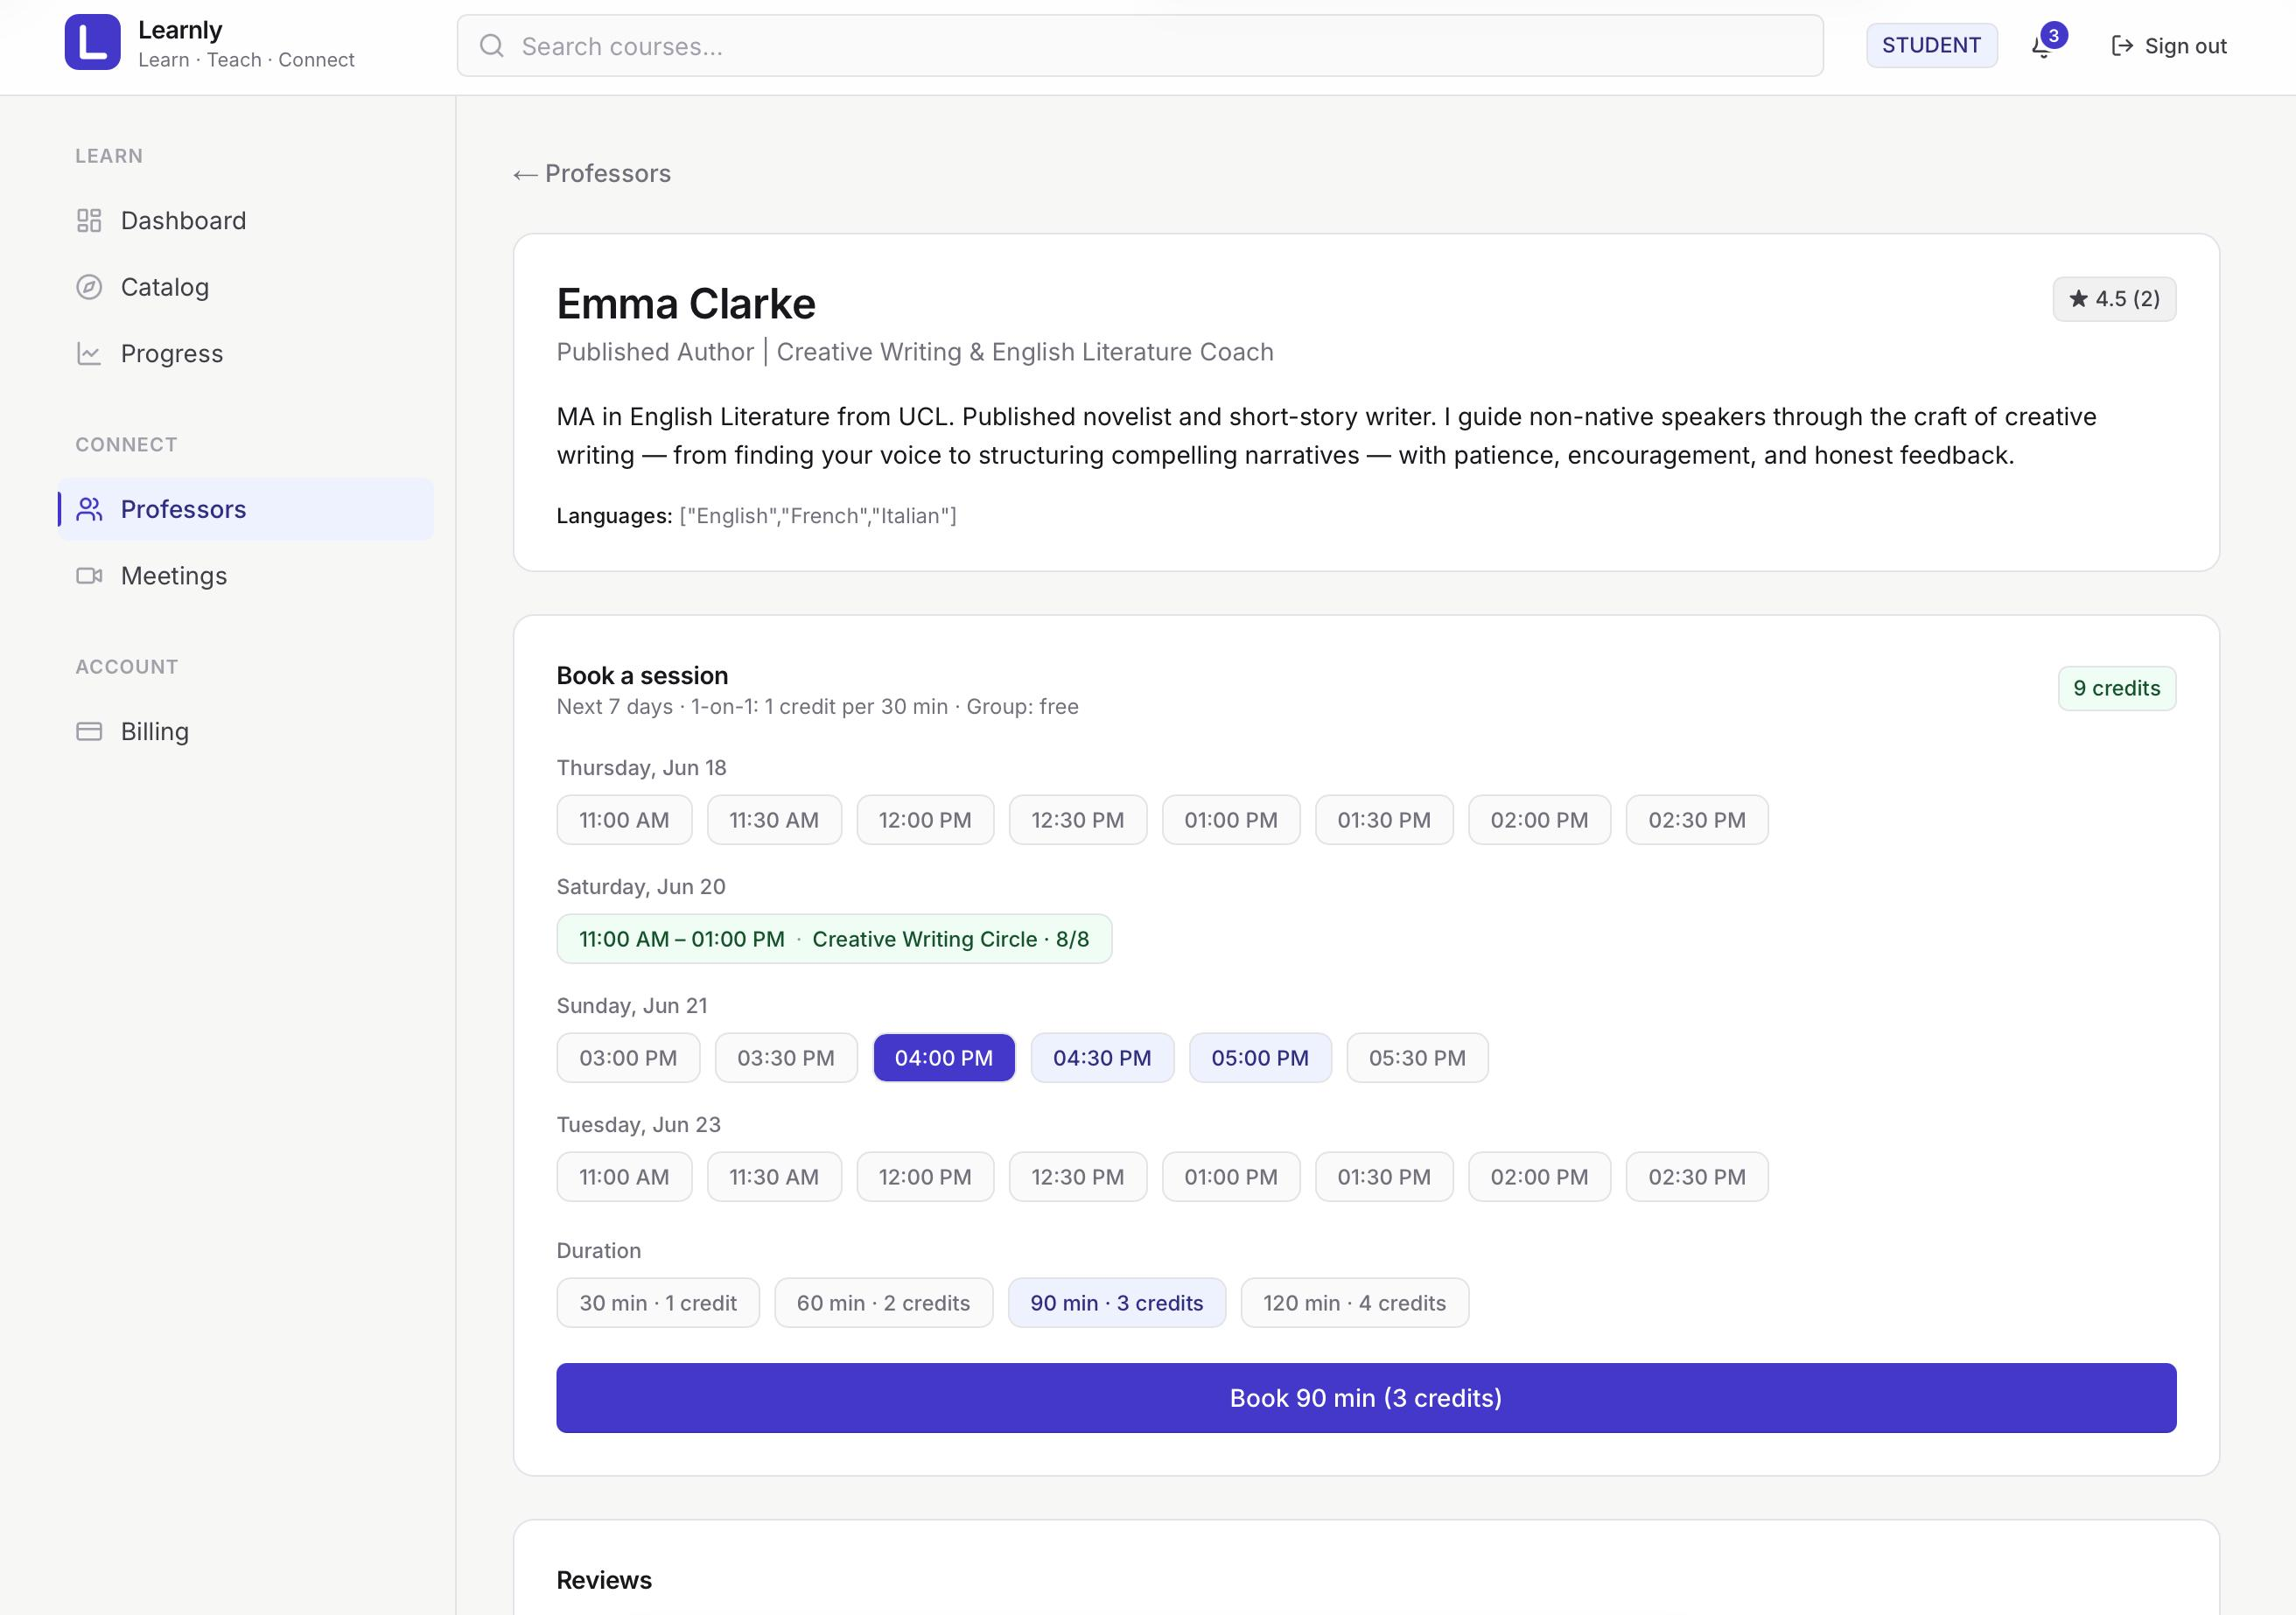
\includegraphics[width=\textwidth]{pics/screenshots/session-booking.jpeg}
    \caption{Rezervarea unei sesiuni cu un profesor}
    \label{fig:session-booking}
\end{figure}

\begin{figure}[htbp]
    \centering
    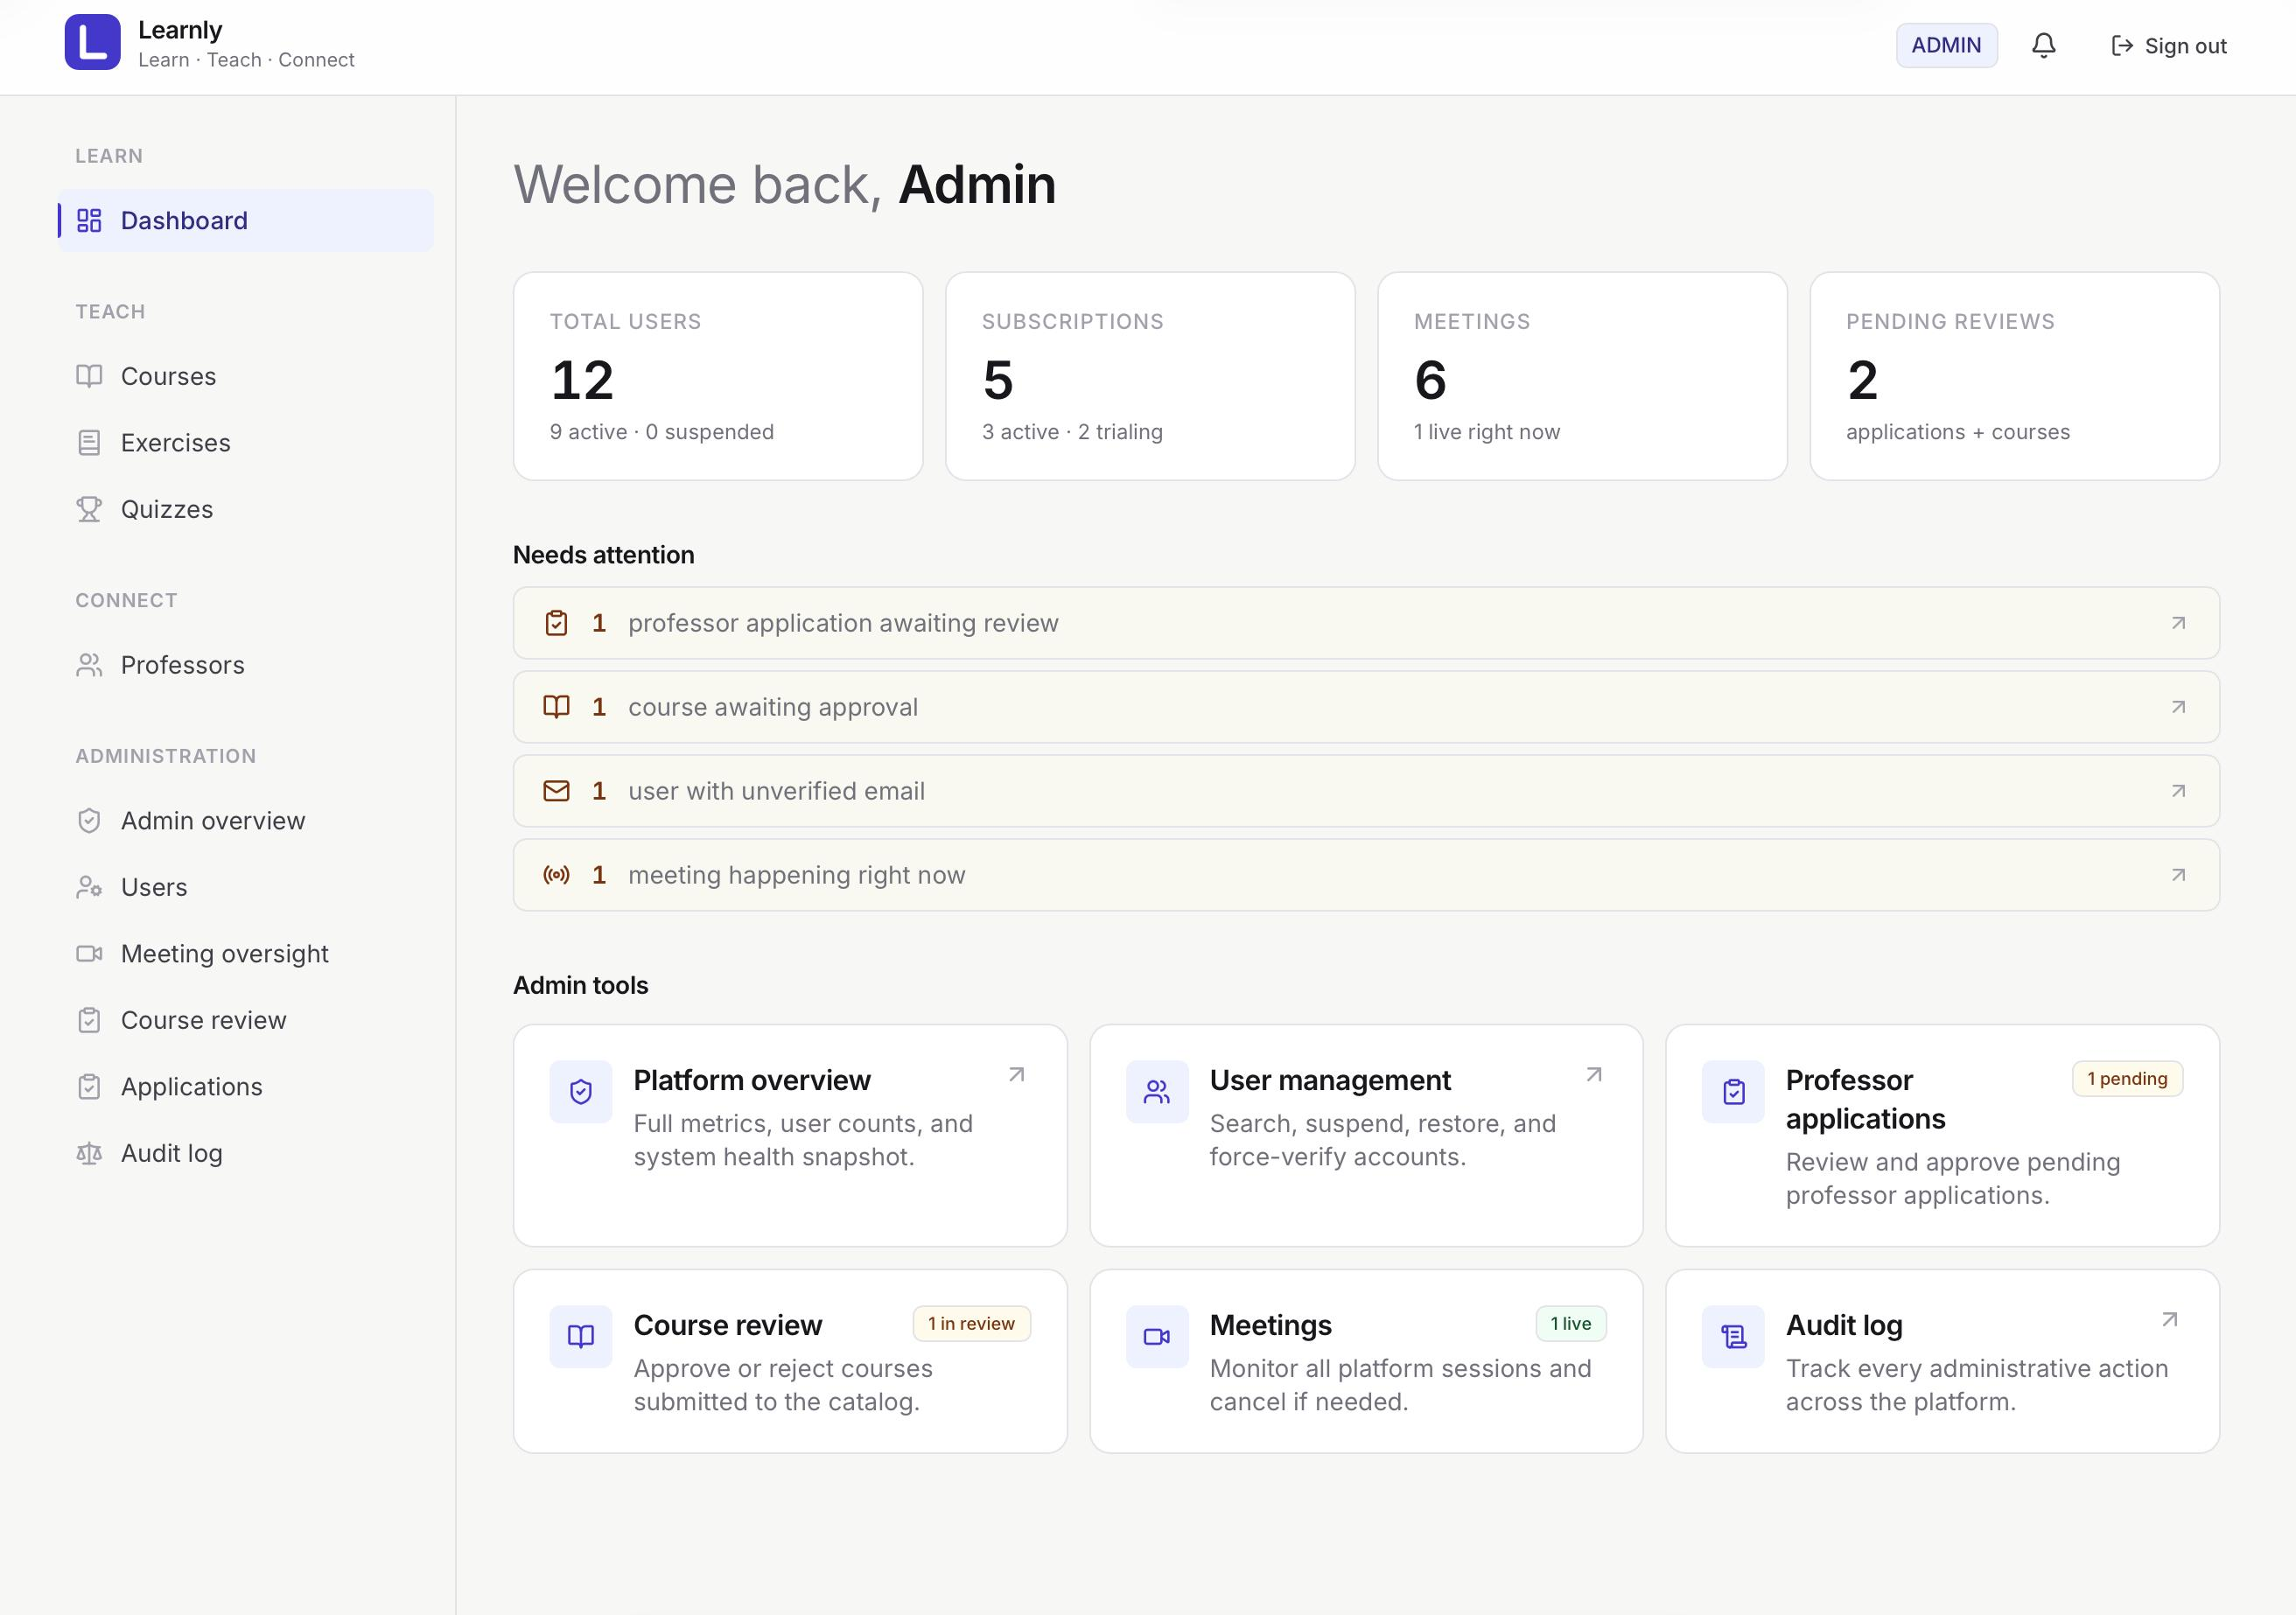
\includegraphics[width=\textwidth]{pics/screenshots/admin-panel.jpeg}
    \caption{Panoul de administrare}
    \label{fig:admin-panel}
\end{figure}

\end{appendices}

\end{document}
